\documentclass[a4paper,draft]{book}
\usepackage[toc,page]{appendix}
%\usepackage[backend=biber,autocite=plain,backref=true]{biblatex}
\usepackage{booktabs} % For enhanced table rules
\usepackage{amsmath, amssymb, amsfonts}
\usepackage{showframe}
\usepackage[dvipsnames]{xcolor}
%\usepackage[top=2cm,bottom=2cm]{geometry}
\usepackage{url}
\usepackage{marginnote}
\usepackage[color=yellow,obeyDraft]{todonotes} % white, lime, pink
\usepackage{nth}

%\usepackage{hyperref}
%\hypersetup{colorlinks, citecolor=blue, filecolor=blue, linkcolor=blue, urlcolor=blue }
%\usepackage[capitalize]{cleveref}  % after hyperref




\usepackage{amsmath, amssymb, amsfonts}
\usepackage{nth}

\usepackage{tikz}
\usetikzlibrary{angles,quotes} % for pic
\tikzset{>=latex} % for LaTeX arrow head
\author{Love}

\usepackage{tocloft}
\DeclareMathOperator{\argmin}{arg\,min} % thin space, limits on side in displays
\DeclareMathOperator{\Cof}{Cof}
\DeclareMathOperator{\rect}{rect}
\DeclareMathOperator{\sign}{sgn}  %DESCRIPTION Sign operator
\DeclareMathOperator{\sinc}{sinc}
\DeclareMathOperator{\tr}{tr}
\DeclareMathOperator{\tri}{tri}
\DeclareMathOperator*{\mini}{\text{minimize}}
\newcommand{\christoffel}[3]{\ensuremath{\Gamma^{#1#2}_{#3}}}
\newcommand{\cross}[2]{\ensuremath{{#1} \times {#2}}}   % alternative: \wedge
\newcommand{\pdv}[2]{\frac{\partial {#1} }{\partial {#2}}} % emulate physics
\newcommand{\Curl}{\boldsymbol{\nabla}\times}
\newcommand{\Div}{\boldsymbol{\nabla}\cdot}
\newcommand{\Grad}{\boldsymbol{\nabla}}
\newcommand{\Lap}{\boldsymbol{\nabla}^2}
\newcommand{\Biharmonic}{\boldsymbol{\nabla}^4}
\newcommand{\pvint}{\mathop{\mathrm{PV}}\!\int}
\newcommand{\ray}[1]{\overset{\rightharpoonup}{#1}}


\newcommand{\abs}[1]{\left\lvert#1\right\rvert}
\newcommand{\norm}[1]{\left\lVert#1\right\rVert}
\newcommand{\del}{\partial}
\newcommand{\eps}{\varepsilon}
\newcommand{\brak}[2]{\left\langle#1,#2\right\rangle}

% other notation for spin, superscript "cross", bmatrix 

\NewDocumentCommand{\fff}{}{\mathrm{I}}







%\addbibresource{/Users/coracle/Documents/VSCODE_LATEX/paraboloid/cones.bib}
\raggedbottom\addtolength{\cftsecnumwidth}{20pt} % Add space for sections
% Add space for subsections (if needed)
\addtolength{\cftsubsecnumwidth}{20pt}

% Table of Contents  widen space for numbers
%\renewcommand{\cftsecnumwidth}{3.2em}%  section
%\renewcommand{\cftsubsecnumwidth}{4.0em} % subsection

\title{Scans of Treatise to LaTeX}
\begin{document}
\maketitle
\tableofcontents

% short version
   \todo[inline]{Skip pages 1--31}
% long version
%  \chapter*{Historical Introduction}
%  \todo[inline]{Skip pages 8--12}
%  \setcounter{page}{12}
%  
Page 13 resist. compression and distortion, he refused to accept the conclusion
from Poisson's theory that the modulus of compression has to the rigidity the
ratio \(5:3\). He pointed out that, if the ratio of these moduluses
could he regarded as infinite, the ratio of the velocities of "longitudinal"
and "transverse" waves would also be infinite, and then, as Green had already
shown, the application of the theory to optics would be facilitated.


The methods of Navier, of Poisson, and of Cauchy's later memoirs lead to
equations of motion containing fewer constants than occur in the equations
obtained by the methods of Green, of Stokes, and of Cauchy's first memoir. The
importance of the discrepancy was first emphasized by Stokes. The questions in
dispute are these — Is elastic aeolotropy to be characterized by 21 constants
or by 15, and is elastic isotropy to be characterized by two constants or one ?
The two theories are styled by Pearson the "multi-constant" theory and the
"rari-constant" theory respectively, and the controversy concerning them has
lasted almost down to the present time. It is to be understood that the
rari-constant equations can be included in the multi-constant ones by equating
certain pairs of the coefficients, but that the rariconstant equations rest
upon a particular hypothesis concerning the constitution of matter, while the
adoption of multi-constancy has been held to imply denial of this hypothesis.
Discrepancies between the results of the two theories can be submitted to the
test of experiment, and it might be thought that the verdict would be final,
but the difficulty of being certain that the tested material is isotropic has
diminished the credit of many experimental investigations, and the tendency of
the multi-constant elasticians to rely on experiments on such bodies as cork,
jelly and india-rubber has weakened their arguments, much of the discussion
has turned upon the value of the ratio of lateral contraction to longitudinal
extension of a bar under terminal tractive load. This ratio is often called
"Poisson's ratio."  Poisson \footnote{Toihniitera.nAVearsoD,HistoryoftheTheoryof
Elasticity, Yo. 1, Cambridge, 1886, p. 496.}> deduced from his theory the
result that this ratio must be \(1/4\). The experiments of Wertheim
\footnote{ Annates de Chimie, t. 23 (1848)}> on glass and brass did not
support this result, and Wertheim proposed to take the ratio to be \(1/3\) —
a value which has no theoretical foundation. The
experimental evidence led Lam in his treatise\footnote{Legons sur la thiorie
mathematique de Velasticite des corps solides, Paris, 1852.}> to adopt the
multi-constant equations, and after the publication of this book they were
generally employed. Saint-Venant, though a firm believer in rari-constancy,

Page 14 of the atoms, we can only invoke the known laws of energy as was done by
Green and Lord Kelvin; and we may place the theory on a firm basis if we
appeal to experiment to support the statement that, within a certain range
of strain, the strain-energy-function is a quadratic function of the
components of strain, instead of relying, as Green did, upon an expansion
of the function in series.

The problem of determining the state of stress and strain within a solid
body which is subjected to given forces acting through its volume and to
given tractions across its surface, or is held by surface tractions so that its
surface is deformed into a prescribed figure, is reducible to the analytical
problem of finding functions to represent the components of displacement.
These functions must satisfy the differential equations of equilibrium at all
points within the surface of the body and must also satisfy certain special
conditions at this surface. The methods which have been devised for integrating
the equations fall into two classes. In one class of methods a special
solution is sought and the boundary conditions are satisfied by a solution in
the form of a series, which may be infinite, of special solutions. The special
solutions are generally expressible in terms of harmonic functions. This class
of solutions may be regarded as constituting an extension of the methods of
expansion in spherical harmonics and in trigonometrical series. In the other
class of methods the quantities to be determined are expressed by definite
integrals, the elements of the integrals representing the effects of
\texttt{singularities}
distributed over the surface or through the volume. This class of solutions
constitutes an extension of the methods introduced by Green in the Theory
of the Potential. At the time of the discovery of the general equations of
Elasticity the method of series had already been applied to astronomical
problems, to acoustical problems and to problems of the conduction of
heat\footnote{See Burkhardt, `Ent wickelungen nach oscillirenden Functionen'
Jahresbericht der Deutschen Mathematiker-Vereinigung, Bd. 10, Heft 2.};
the method of singularities had not been
invented\footnote{It was invented by Green, An Essay on the Application of
Mathematical Analysis to the Theories of Electricity and Magnetism, Nottingham,
1828. Reprinted in Mathematical Papers of the late George Green, London,
1871.}. The application of the method of series to problems of equilibrium of
elastic solid bodies was initiated
\setcounter{footnote}{38}
by Lamé and Clapeyron\footnote{See footnote 39}. They considered the case of a
body bounded by an unlimited plane to which pressure is applied according to an
arbitrary law.
\setcounter{footnote}{59}
Lamé\footnote{Journal de Math. (Liouville), t. 19 (1854).}
later considered the problem of a body bounded by a spherical surface
and deformed by given surface tractions. The problem of the plane is
essentially that of the transmission into a solid body of force applied locally
to a small part of its surface. The problem of the sphere has been developed
by Lord
Kelvin\footnote{Phil. Trans. Boy. Soc, vol. 153 (1863). See also Mathematics
and Phys. Papers, vol. 3 (Cambridge, 1890), p. 351, and Kelvin and Tait, Nat.
Phil., Part 2.} who sought to utilize it for the purpose of investigating the
rigidity of the Earth\footnote{Brit. Assoc. Rep. 1876, Math, and Phys. Papers,
vol. 3, p. 312.}, and by G. H. Darwin in connexion with other problems of
cosmical
physics\footnote{Phil. Trans. Roy. Soc, vol. 170 (1879), and vol. 173 (1882).
Reprinted in G. H. Darwin's Scientific Papers, vol. 2, Cambridge 1908, pp. 1, 459.}.
The serial solutions employed are expressed
in terms of spherical harmonics. Solutions of the equations in cylindrical
coordinates can be expressed in terms of Bessel's
functions\footnote{L. Pochhammer, J.f. Math. (Crelle), Bd. 81 (1876), p. 38.},
but, except for spheres and cylinders, the method of series has not been employed very
successfully. The method of singularities was first applied to the theory of
Elasticity by E. Betti\footnote{II Nuovo Cimento (Ser. 2), tt. 6—10 (1872 et seq.)},
who set out from a certain reciprocal theorem of the
type that is now familiar in many branches of mathematical physics. From
this theorem he deduced incidentally a formula for determining the average
strain of any type that is produced in a body by given forces. The method
of singularities has been developed chiefly by the elasticians of the Italian
school. It has proved more effective than the method of series in the solution
of the problem of transmission of force. The fundamental particular solution
which expresses the displacement due to force at a point in an indefinitely
extended solid was given by Lord
Kelvin\footnote{Sir W. Thomson, Cambridge and Dublin Math. J., 1848, reprinted in Math
and Phys. Papers, vol. 1, p. 97}.  It was found at a later date by J.
Boussinesq\footnote{For Boussinesq's earlier researches in
regard to simple solutions, see Paris, C. R., tt. 86—88 (1878—1879)
and tt. 93—96 (1881—1883). A more complete account is given in his book,
Applications des potentiels à l'étude de l'équilibre et du mouvement
des solides elastiques, Paris, 1885.}
along with other particular solutions, which can, as a matter
of fact, be derived by synthesis from it. Boussinesq's results
led him to a solution of the problem of the plane, and to a theory of
``local perturbations'' according to which the effect of force applied
in the neighbourhood of any point of a body falls off very rapidly as
the distance from the point increases, and the application of an
equilibrating system of forces to a small part of a body produces an
effect which is negligible at a considerable distance from the part.
To estimate the effect produced at a distance by forces applied
near a point, it is not necessary to take into account the mode of
application of the forces but only the statical resultant and moment.
The direct method of integration founded upon Betti's reciprocal
theorem was applied to the problem of the plane by V.
Cerruti\footnote{Rome, Acc. Lincei, Mem.\ fis.\ mat., 1882.
}. Some of the results were found independently by Hertz, and
led in his hands to a theory of impact and a theory of
hardness\footnote{J. f. Math. (Crelle), Bd. 92 (1882), and Verhandlungen
des Vereins zur Beförderung des Gewerbefleisses, Berlin, 1882. The memoirs
are reprinted in Ges. Werke von Heinrich Hertz, Bd. 1, Leipzig, 1895, pp. 155 and 174.
}.

A different method for determining the state of stress in a body
has been developed from a result noted by G. B.
Airy\footnote{70 Brit. Assoc. Rep. 1862, and Phil. Trans. Roy. Soc, vol. 153
(1863), p. 49}.  He observed that, in the case
of two dimensions, the equations of equilibrium of a body deformed by surface
tractions show that the stress-components can be expressed as partial differential
coefficients of the second order of a single function.
Clerk Maxwell\footnote{71 Edinburgh Roy. Soc. Trans., vol. 26 (1870). Reprinted in Maxwell's
Scientific Papers, vol. 2, p. 161.} ``extended the
result to three dimensions, in which case three such ``stress-functions'' are
required. It appeared later that these functions are connected by a rather
complicated system of, differential equations\footnote{72 W. J. Ibbetson, An Elementary
Treatise on the Mathematical Theory of
perfectly Elastic Solids, London, 1887.}. The stress-components must
in fact be connected with the strain-components by the stress-strain relations,
and the strain-components are not independent; but the second differential
coefficients of the strain-components with respect to the coordinates are
connected by a system of linear equations, which are the conditions necessary to
secure that the strain-components shall correspond with a displacement, in
accordance with the ordinary formulas connecting strain and
displacement\footnote{73 Saint-Venant gave the identical relations between
strain-components in his edition of Navier's Résumé des Leçons sur I'application
de la Mécanique, Paris, 1864, Appendice 3}.
It is possible by taking account of these relations to obtain a complete system
of equations which must be satisfied by stress-components, and thus the way
is open for a direct determination of stress without the intermediate steps of
forming and solving differential equations to determine the components of
displacement\footnote{J. H. Michell, London Math. Soc. Proc, vol. 31 (1900), p. 100.}.
In the case of two dimensions the resulting equations are of a
simple character, and many interesting solutions can be obtained.

The theory of the free vibrations of solid bodies requires the integration
of the equations of vibratory motion in accordance with prescribed boundary
conditions of stress or displacement. Poisson\footnote{36} gave the solution of the
problem of free radial vibrations of a solid sphere, and Clebsch\footnote{53}
founded the general theory on the model of Poisson's solution. This theory
included the extension of the notion of ``principal coordinates'' to systems
with an infinite number of degrees of freedom, the introduction of the
corresponding ``normal functions'' and the proof of those properties of these
functions upon which the expansions of arbitrary functions depend. The
discussions which had taken place before and during the time of Poisson
concerning the vibrations of strings, bars, membranes and plates had prepared
the way for Clebsch's generalizations. Before the publication of Clebsch's
treatise a different theory had been propounded by Lamé\footnote{49}.
Acquainted with Poisson's discovery of two types of waves, he concluded that
the vibrations of any solid-body must fall into two corresponding classes, and
he investigated the vibrations of various bodies on this assumption. The fact
that his solutions do not satisfy the conditions which hold at the boundaries
of bodies free from surface traction is a sufficient disproof of his theory;
but it was finally disposed of when all the modes of free vibration of a
homogeneous isotropic sphere were determined, \setcounter{footnote}{74}
and it was proved that the classes into which they fall do not verify
Lamé's supposition. The analysis of the general problem of the vibrations
of a sphere was first completely given by 
P. Jaerisch\footnote{75 J.f. Math. (Crelle), Bd. 88 (1880)},
who showed that the
solution could be expressed by means of spherical harmonics and certain
functions of the distance from the centre of the sphere, which are practically
Bessel's functions of order integer \(+1/2\). This result was obtained
independently by H. Lamb\footnote{76 London Math. Soc. Proc, vol. 13 (1882)},
who gave an account of the simpler modes of vibration
and of the nature of the nodal division of the sphere which occurs when any
normal vibration is executed. He also calculated the more important roots
of the frequency equation. 
L. Pochhammer\footnote{77 J. f. Math. (Crelle), Bd. 81 (1876), p. 324
}has applied the method of normal
functions to the vibrations of cylinders, and has found modes of vibration
analogous to the known types of vibration of bars.

The problem of tracing, by means of the equations of vibratory motion,
the propagation of waves through an elastic solid medium requires investigations
of a different character from those concerned with normal modes of
vibration. In the case of an isotropic medium
Poisson\footnote{78 Paris, Mém.\ de l'Acad.,t. 10 (1831).}
and Ostrogradsky\footnote{79 St Petersburg, Mém.\ de I' Acad., t. 1 (1831).} adopted
methods which involve a synthesis of solutions of simple harmonic
type, and obtained a solution expressing the displacement at any time in
terms of the initial distribution of displacement and velocity. The investigation
was afterwards conducted in a different fashion by
Stokes\footnote{80. `On the Dynamical Theory of Diffraction'
Cambridge Phil. Soc. Trans., vol. 9 (1849). Reprinted in Stokes's Math, and Phys.
Papers, vol. 2 (Cambridge, 1883)}, who showed
that Poisson's two waves are waves of irrotational dilatation and waves of
equivoluminal distortion, the latter involving rotation of the elements of the
medium. Cauchy\footnote{41} and
\setcounter{footnote}{80}
Green\footnote{81 Cambridge Phil. Soc. Trans., vol. 7 (1839).  Reprinted in
Green's Mathematical Papers, p. 293} discussed the propagation of plane waves
through a crystalline medium, and obtained equations for the velocity of
propagation in terms of the direction of the normal to the wave-front. In general
the wave-surface has three sheets; when the medium is isotropic all the sheets
are spheres, and two of them are coincident. Blanchet\footnote{82 82 J. de Math.
(Liouville), t. 5 (1840), t. 7 (1842).
}
extended Poisson's
results to the case of a crystalline medium. Christoffel\footnote{83 83 Ann.\ di Mat.
(Ser. 2), t. 8 (1877).Reprinted in E. B. Christoffel Ges.\ math. Abhandlmgen, Bd. 2,
p. 81, Leipzig 1910.} discussed the advance
through the medium of a surface of discontinuity. At any instant,
the surface separates two portions of the medium in which the displacements are
expressed by different formulae; and Christoffel showed that the surface moves
normally to itself with a velocity which is determined, at any point, by the
direction of the normal to the surface, according to the same law as holds


%  \todo[inline]{Skip pages 17--31}

\setcounter{page}{32}
\chapter{Analysis of Strain}
\section{Extension}
%\chapter{Analysis of Strain} \setcounter{page}{32} \section{Extension}
Whenever, owing to any cause, changes take place in the relative positions 
of the parts of a body the body is said to be \textit{strained}. A very simple 
example of a strained body is a stretched bar. Consider a bar of square 
section suspended vertically and loaded with a weight at its lower end. 
Let a line be traced on the bar in the direction of its length, let two points of 
the line be marked, and let the distance between these points be measured. 
When the weight is attached the distance in question is a little greater than 
it was before the weight was attached. Let \(l_o\) be the length before stretching, and
\(l\) the length when stretched. Then \((l-l_o)/l_o\), is a number (generally a 
very small fraction) which is called the \textit{extension} of the line in question. If 
this number is the same for all lines parallel to the length of the bar, it may 
be called \textit{the extension of the bar}. A steel bar of sectional area \(1~in^2\)
\(=6.4515~cm^2\) loaded with 1 ton \(= 1016.05 kg\) will undergo an extension of about
\(7 \times 10^{-5}\). It is clear that for the measurement of such 
small quantities as this rather elaborate apparatus and refined methods of 
observation are required \footnote{See, for example, Ewing, Strength of
Materials, Cambridge, 1899, pp. 73 et seq., or G. P. C. Searle, Experimental
Elasticity, Cambridge, 1908.} Without attending to methods of measurement 
we may consider a little more in detail the state of strain in the stretched 
bar. Let \(e\) denote the extension of the bar, so that its length is increased in 
the ratio \(1+e:1\), and consider the volume of the portion of the bar
contained between any two marked sections. This volume is increased by
stretching the bar, but not in the ratio \(1+e:1\) . When the bar is stretched
longitudinally, it contracts laterally. If the linear lateral contraction is
\(e^{\prime}\), the sectional area is diminished in the ratio
\((1-e^{\prime})^2:1\), and the volume in question is increased in the ratio
\((1+e)(1-e^{\prime})^2:1\).  In the case of a bar under tension,
\(e^{\prime}\) is a certain multiple of \(e\), say \(\sigma e\)
\footnote{Kirchhoff's notation, Poisson's ratio, Filon used \(\nu\).},
and \(\sigma\) is about \(1/3\) for very many materials. If \(e\)
is very small and \(e^2\) is neglected, the areal contraction \(2 \sigma e\), 
\[
(1-2 \sigma e)(1+e) = 1 + e - 2 \sigma e  = 1+ e(1-2 \sigma),
\]
and, the cubical dilatation is \((1-2 \sigma) e\).

For the analytical description of the state of strain in the bar we should 
take an origin of coordinates \(x\), \(y\), \(z\) on the axis, and measure the
coordinate \(z\)

along the length of the bar. Any particle of the bar which has the coordinates
\(x\), \(y\), \(z\)
when the weight is not attached will move after the attachment 
of the weight into a new position. Let the particle which was at the origin 
move through a distance
\(z_o\), then the particle which was at
\((x,y,z)\)
moves to 
the point of which the coordinates are 
\[
(x(1-\sigma e), \quad y(1-\sigma e), \quad z_o + (z-z_o) (1+ e)).
\]
The state of strain is not very simple. If lateral forces could be applied to 
the bar to prevent the lateral contraction the state of strain would be very 
much simplified. It would then be described as a \textit{simple extension}. 

\section{Pure  shear}
As a second example of strain let us suppose that lateral forces are applied 
to the bar so as to produce extension of amount
\(\epsilon_1\) of lines parallel to the axis of \(x\) and
extension of amount \(\epsilon_2\) of lines parallel to the axis \(y\), and that 
longitudinal forces are applied, if any are required, to prevent any extension 
or contraction parallel to the axis of \(z\). The particle which was at
\((x, y, z)\) will move to \((x+\epsilon_1 x,y+\epsilon_2 y, z)\)
and the area of the section will be increased in the ratio
\((1+\epsilon_1)(1+\epsilon_2):1\).
If \(\epsilon_1\) and \(\epsilon_2\)
are related so that this ratio is equal to unity,
\[
(1+\epsilon_1)(1+\epsilon_2)=1,
\]
there will be no change in the area of the section or in the volume of any
portion of the bar, but the shape of the section will be distorted.  Either
\(\epsilon_1\) or \(\epsilon_2\) is then negative, or there is contraction of
the corresponding set of lines.  The strain set up in the bar is called
\textit{pure shear}.  Fig. 1 below shows a square \(ABCB\) distorted by pure
shear into a rhombus \(A'B'C'D'\) of the same area. 

\section{Simple shear}
As a third example of strain let us suppose that the bar after being distorted
by pure shear is turned bodily about its axis. We suppose that the axis of
\(x\) is the direction in which contraction takes place, and we put 
\[
\epsilon_2 - \epsilon_1 = 2 \tan \alpha.
\]

Then we can show that, if the rotation is of amount \(\alpha\) in the sense
from \(y\) to \(x\), the position reached by any particle is one that could
have been reached by the sliding of all the particles in the direction of a
certain line through distances proportional to the distances of the particles
from a certain plane containing this line. 

Since \((1+\epsilon_1)(1+\epsilon_2)=1\), and \(\epsilon_2 -\epsilon_1 = 2 \tan
\alpha\), we have 
\[
1 + \epsilon_1 = \sec(\alpha ) - \tan(\alpha ), \quad
1 + \epsilon_2 = \sec(\alpha ) + \tan(\alpha ).
\] 
By the pure shear, the particle which was at
\((x, y)\)
will move to
\((x_1,y_1)\), where 
\[
\begin{bmatrix}
x_1\\
y_1 
\end{bmatrix}=
\begin{bmatrix}
(\sec(\alpha ) - \tan(\alpha ))x\\
(\sec(\alpha ) + \tan(\alpha ))y 
\end{bmatrix}
\] 
and by the rotation it is moved again to
\((x_2,y_2)\), where
\[
\begin{bmatrix} x_2\\ y_2 \end{bmatrix}=
\begin{bmatrix}
\cos(\alpha ) & \sin(\alpha )\\
-\sin(\alpha ) & \cos(\alpha )
\end{bmatrix}
\begin{bmatrix} x_1\\ y_1 \end{bmatrix}.
\] 
so that we have
\[
\begin{bmatrix} x_2\\ y_2 \end{bmatrix}=
\begin{bmatrix} x\\ y \end{bmatrix}+ \tan(\alpha) 
\begin{bmatrix}
-\cos(\alpha )  & 1+\sin(\alpha )\\
-1+\sin(\alpha )& \cos(\alpha )
\end{bmatrix}
\begin{bmatrix}
x\\
y
\end{bmatrix}.
\]

Now, writing 
\(\beta\) for 
\(\frac{1}{2}\pi-a\), we have 
\[
\begin{bmatrix} x_2\\ y_2 \end{bmatrix}=
\begin{bmatrix} x\\ y \end{bmatrix}+ 
2 \tan(\alpha) \left(
-x \sin \frac{\beta}{2} + y \cos\frac{\beta}{2}
\right)
\begin{bmatrix}
\cos(\beta/2) \\
\sin(\beta/2) 
\end{bmatrix}
\]
and we can observe that 
\[
\begin{aligned}
x_2 \cos \frac{\beta}{2} + y_2 \sin \frac{\beta}{2}=&
x \cos \frac{\beta}{2} + y \sin \frac{\beta}{2}
+ 2 \tan(\alpha) \left(
-x \sin \frac{\beta}{2} + y \cos\frac{\beta}{2} \right), \\
-x_2 \sin \frac{\beta}{2} + y_2 \cos\frac{\beta}{2}&=
-x\sin\frac{1}{2}\beta+y\cos\frac{1}{2}\beta.
\end{aligned}
\]
Hence, taking axes of \(X\) and \(Y\) which are obtained from those of
\(x\) and \(y\) by a rotation through 
\(\frac{\pi}{4}\pi - \frac{\alpha}{2}\) in the sense from
\(x\) towards \(y\), we see that the particle which was at
\((X, Y)\) is moved by the pure shear followed by 
the rotation to the point
\((X_2, Y_2)\), where
\[
\begin{bmatrix}
X_2 \\
Y_2
\end{bmatrix} =
\begin{bmatrix}
1 & 2\tan\alpha \\
0 &  1
\end{bmatrix}
\begin{bmatrix}
X \\
Y
\end{bmatrix}
.\]

Thus every plane of the material which is parallel to the plane of
\((X, z)\) slides 
along itself in the direction of the axis of
\(X\) through a distance proportional 
to the distance of the plane from the plane of
\((X, z)\). The kind of strain just 
described is called a \textit{simple shear}, the angle \(\alpha\)
is the \textit{angle of the shear}, 
and \(2 \tan \alpha\) is the \textit{amount of the shear}.

\begin{figure}[!h]
\caption{Shear}
 \label{fig:1}
\end{figure}
Fig. 1 shows a square \(ABCB\) distorted by pure shear into a rhombus
\(A'B'C'D'\) of the same area, which is then rotated into the position
\(A''B''C''D''\). The angle of the shear is \(A'OA''\), and the angle \(AOX\)
is half the complement of this angle.  The lines \(AA'',BB'',CC'',DD''\) are
parallel to \(OX\) and proportional to their distances from it.

We shall find that all kinds of strain can be described in terms of
simple extension and simple shear, but for the discussion of complex
states of strain and for the expression of them by means of simpler
strains we require a general kinematical theory\footnote{The greater
  part of the theory is due to Cauchy (see Introduction). Some
  improvements were made by Clebsch in his treatise of 1862, and others
  were made by Kelvin and Tait, Nat. Phil. Part I.}

\section{Displacement.} % 4

We have, in every case, to distinguish two states of a body a first
state and a second state. The particles of the body pass from their
positions in the first state to their positions in the second state by a
displacement. The displacement may be such that the line joining any two
particles of the body has the same length in the second state as it has
in the first; the displacement is then one which would be possible in a
rigid body. If the displacement alters the length of any line, the
second state of the body is described as a \textit{strained state}, and
then the first state is described as the \textit{unstrained state}.

In what, follows we shall denote the coordinates of the point occupied
by a particle, in the unstrained state of the body, by x, y, z, and the
coordinates of the point occupied by the same particle in the strained
state by \(x + u, y+v, z + w.\) Then \(u, v, w\) are the projections on
the axes of a vector quantity --- the displacement. We must take
\(u, v, w\) to be continuous functions of \(x, y, z,\) and we shall in
general assume that they are analytic functions.

It is clear that, if the displacement (u, v, w) is given, the strained
state is entirely determined; in particular, the length of the line
joining any two particles can be determined.

\section{Displacement in simple extension and simple shear.} % 5
The displacement in a simple extension parallel to the axis of x is
given by the equations \(u=ex, v=0, w=0,\) where e is the amount of
the extension. If e is negative there is contraction.

The displacement in a simple shear of amount (=2 tan a), by which lines
parallel to the axis of x slide along themselves, and particles in any
plane parallel to the plane of (X, y) remain in that plane, is given by
the equations \(u=s y, v=0, w=0.\)

In Fig. 2, \(A B\) is a segment of a line parallel to the axis of \(x\), which
subtends an angle \(2 a\) at \(O\) and is bisected by \(O y\). By the simple
shear particles lying on the line \(O A\) are displaced so as to lie on \(O
B\). The particle at any point \(P\) on \(A B\) is displaced to \(Q\) on \(A
B\) so that \(P Q=A B\), and the particles on \(O P\) are displaced to points
on \(O Q\). A parallelogram such as \(O P N M\) becomes a parallelogram such as
\(O Q K M\).


\todo[inline]{Imagine Fig 2 is here.}
\begin{figure}[!h]
\centering
  %\usepackage{tikz}
  %\usetikzlibrary{angles,quotes} % for pic
  %\tikzset{>=latex} % for LaTeX arrow head
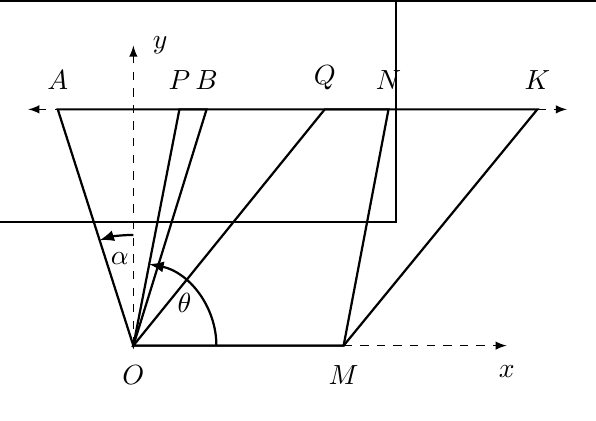
\begin{tikzpicture}[scale=1.5]
  % Define the coordinates

  \coordinate (O) at (0,0);
  \coordinate (M) at (1.78,0);
  \coordinate (X) at (3.16,0);

  \coordinate (Left) at (-0.89,2); 
  \coordinate (Right) at (3.67,2); 
  \coordinate (Y) at (0,2.54);
  %  A < P < B < Q < N < K
  \coordinate (A) at (-0.64,2);

  \coordinate (P) at (0.39,2); 
  \coordinate (B) at (0.62,2); 

  \coordinate (Q) at (1.62,2);
  \coordinate (N) at (2.16,2);  % N - P = M - O
  \coordinate (K) at (3.42,2);  % K -Q  = N -P

  % Draw the closed polygon (triangle)
  \draw[thick] (O) -- (M) -- (N) -- (P) -- cycle;
  \draw[thick] (O) -- (M) -- (K) -- (Q) -- cycle;
  \draw[thick] (O) -- (B) -- (A) -- cycle;

  \draw[->,dashed] (O) -- (Y); 
  \draw[->,dashed] (M) -- (X); 
  \draw[<-,dashed] (Left) -- (A); 
  \draw[dashed,->] (K) -- (Right); 
  \draw pic ["$\theta$",draw,->,thick,angle radius=30, angle eccentricity=0.8,] {angle= M--O--P};
  \draw pic ["$\alpha$",draw,->,thick,angle radius=40, angle eccentricity=0.8] {angle= Y--O--A};

  % Draw and label the vertices
  \node[label=below :$O$] at (O) {};
  \node[label=below :$M$] at (M) {};
  \node[label=below:$x$] at (X) {};
  \node[label=above:$A$] at (A) {};
  \node[label=right:$y$] at (Y) {};
  \node[label=above:$P$] at (P) {};
  \node[label=above:$B$] at (B) {};
  \node[label=above:$Q$] at (Q) {};
  \node[label=above:$N$] at (N) {};
  \node[label=above:$K$] at (K) {};
\end{tikzpicture}
 \caption{Exact Shear}
 \label{fig:2}
\end{figure}
If the angle \(x O P=\theta\) we may prove that
\[
\tan P O Q=\frac{2 \tan \alpha \tan ^2 \theta}{\sec ^2 \theta+2 \tan \alpha
\tan \theta}, \quad \tan x O Q=\frac{\tan \theta}{1+2 \tan \alpha \tan \theta}
\]
In particular, if \(\theta=\frac{1}{2} \pi, \cot x O Q=s\), so that, if \(s\)
is small, it is the complement of the angle in the strained state between two
lines of particles which, in the unstrained state, were at right angles to each
other.


\section{Homogeneous strain.} % 6
In the cases of simple extension and simple shear, the component displacements
are expressed as linear functions of the coordinates. In general, if a body is
strained so that the component displacement can be expressed in this way, the
strain is said to be \textit{homogeneous}.

Let the displacement corresponding with a homogeneous strain be given by the
equations
\[
u=a_{11} x+a_{12} y+a_{13} z, \quad v=a_{21} x+a_{22} y+a_{23} z, \quad
w=a_{31} x+a_{32} y+a_{33} z .
\]
Since \(x, y, z\) are changed into \(x+u, y+v, z+w\), that is, are transformed
by a linear substitution, any plane is transformed into a plane, and any
ellipsoid is transformed, in general, into an ellipsoid. We infer at once the
following characteristics of homogeneous strain: 
\begin{itemize}
\item[(i)] Straight lines remain straight. 
\item[(ii)] Parallel straight lines remain parallel. 
\item[(iii)] All straight lines in the same direction are extended, or
contracted, in the same ratio. 
\item[(iv)] A sphere is transformed into an ellipsoid, and any three orthogonal
diameters of the sphere are transformed into three conjugate diameters of the
ellipsoid. 
\item[(v)] Any ellipsoid of a certain shape and orientation is transformed into
a sphere, and any set of conjugate diameters of the ellipsoid is transformed
\end{itemize}

\todo[inline]{missing, not started, not scanned 37--45 art 7--14}
\setcounter{section}{14}
\setcounter{equation}{13}
The relative displacement corresponding with plane strain is parallel to the
plane of the strain; or we have \(w=\) const., while \(u\) and \(v\) are
functions of \(x\) and \(y\) only. The axis of the resultant rotation is normal
to the plane of the strain. The cubical dilatation, \(\Delta\), and the
rotation, \(\varpi\), are connected with the displacement by the equations
\[
\Delta=\frac{\partial u}{\partial x}+\frac{\partial v^{\prime}}{\partial
y^{\prime}}, \quad 2 w=\frac{\partial v}{\partial x}-\frac{\partial u}{\partial
y}.
\]
We can have states of plane strain for which both \(\Delta\) and \(\varpi\)
vanish; the strain is pure shear, i.e. shearing strain combined with such a
rotation that the principal axes of the strain retain their primitive
directions. In any such state the displacement components \(v, u\) are
conjugate functions of \(x\) and \(y\), or \(v+\imath u\) is a function of the
complex variable \(x+\imath y\).

\section{Relations connecting the dilatation, the rotation and the displacement.} %15
The cubical dilatation \(\Delta\) is connected with the displacement
\((u, v, w)\) by the equation
\[
\Delta=\frac{\partial u}{\partial x}+\frac{\partial v}{\partial y}+
\frac{\partial w}{\partial z}.
\]
A scalar quantity derived from a vector by means of this formula is described
as the \textit{divergence} of the vector. We write
\begin{equation}\label{eq:14}
\Delta=\operatorname{div}(u, v, w).
\end{equation}
This relation is independent of coordinates, and may be expressed as
follows: - Let any closed surface \(S\) be drawn in the field of the vector, and
let \(N\) denote the projection of the vector on the normal drawn outwards at
any point on \(S\), also let \(d \tau\) denote any element of volume within
\(S\), then
\begin{equation}\label{eq:15}
\iint N d S=\iiint \Delta d \tau,
\end{equation}
the integration on the right-hand side being taken through the volume within
\(S\), and that on the left being taken over the
surface \(S\)\footnote{The result is a particular case of the theorem known as
'Green's theorem.' See Ency: \(d\). math. Wiss. II. A 2, Nos. 45-47.}.

The rotation \(\left(\varpi_x, \varpi_y, \varpi_z\right)\) is connected with
the displacement \((u, v, w)\) by the equations
\[
2 \varpi_x=\frac{\partial w}{\partial y}-\frac{\partial v}{\partial z}, \quad
2 \varpi_y=\frac{\partial u}{\partial z}-\frac{\partial w}{\partial x}, \quad
2 \varpi_z=\frac{\partial v}{\partial x}-\frac{\partial u}{\partial y} .
\]

A vector quantity derived from another vector by the process here indicated is
described as the curl of the other vector. We write
\begin{equation}\label{eq:16}
2\left(\varpi_x, \varpi_y, \varpi_z\right)=\operatorname{curl}(u, v, w).
\end{equation}
This relation is independent of coordinates\footnote{It is assumed that the
axes of \(x, y, z\) form a right-handed system.  If a transformation to a
left-handed system is admitted a convention must be made as to the sign of
the curl of a vector.}, and may be expressed as
follows:-Let any closed curve \(s\) be drawn in the field of the vector, and
let any surface \(S\) be described so as to have the curve \(s\) for an edge;
let \(T\) be the resolved part of the vector \((u, v, w)\) along the tangent at
any point of \(s\), and let \(2 \varpi_\nu\) be the projection of the vector
\(2\left(\varpi_x, \varpi_y, \varpi_z\right)\) on the normal at any point of
\(S\), then
\begin{equation}\label{eq:17}
\int T d s=\iint 2 \varpi_\nu d S,
\end{equation}

\todo[inline]{missing, not started, p 47--50, art 15--18, is scanned}
\todo[inline]{skip p 47--50, art 15--18 to p51 Art 18 Determined by Strain}
\setcounter{section}{18}
\setcounter{equation}{27}
would not express the strain in the body correctly, and the terms of
(27) that contain \(p, q, r\) would not represent a displacement
possible in a rigid body. Bearing this restriction in mind, we conclude
that, if the six components of strain are given, the corresponding
displacement is arbitrary to the extent of an additional displacement of
the type expressed by (27); but, if we impose 
six independent conditions,
such as that, at the origin, the displacement \((u, v, w)\) and the rotation
\(\left(\varpi_x, \varpi_y, \varpi_z\right)\) vanish, or again that, at the
same point
\begin{equation}\label{eq:28}
u=0,v=0,w=0, \frac{\partial u}{\partial z}=0,
\frac{\partial v}{\partial z}=0, \frac{\partial v}{\partial x}=0,
\end{equation}
the expression for the displacement with given strains will be unique.
The particular set of equations (\ref{eq:28}) indicate that one point of the body
(the origin), one linear element of the body (that along the axis of
\(z\) issuing from the origin) and one plane-element of the body (that
in the plane of \(z, x\) containing the origin) retain their positions
after the strain. It is manifestly possible, after straining a body in
any way, to bring it back by translation and rotation so that a given
point, a given linear element through the point and a given
plane-element through the line shall recover their primitive positions.

\section{Curvilinear orthogonal coordinates}
For many problems it is convenient to use systems of curvilinear
coordinates\footnote{The theory is due to Lamé. See his
Leçons sur les coordonnées curvilignes, Paris, 1859.}
instead of the ordinary Cartesian coordinates. These may be
introduced as follows: Let \(f(x, y, z)=\alpha \), some constant,
be the
equation of a surface. If \(\alpha \) is allowed to vary we obtain a
family of surfaces. In general one surface of the family will pass
through a chosen point, and a neighbouring point will in general lie
on
a neighbouring surface of the family, so that \(\alpha \) is a function
of \(x, y, z\), viz., the function denoted by \(f\). If
\(\alpha+d \alpha \) is the parameter of that surface of the family which
passes through \((x+d x, y+d y, z+d z)\), we have
\[
d \alpha=\frac{\partial f}{\partial x} d x+\frac{\partial f}{\partial y} d y+
\frac{\partial f}{\partial z} d z=\frac{\partial \alpha}{\partial x} d x+
\frac{\partial \alpha}{\partial y} d y+\frac{\partial \alpha}{\partial z} d z.
\]

If we have three independent families of surfaces given by the equations
\[f_1(x, y, z)=\alpha, \quad f_2(x, y, z)=\beta, \quad f_3(x, y, z)=\gamma,\]
so that in general one surface of each family passes through a chosen
point, then a point may be determined by the values of
\(\alpha, \beta, \gamma \) which belong to the surfaces that pass through
it\footnote{The determination of the
point may not be free from ambiguity, e.g., in elliptic coordinates, an
ellipsoid and two confocal hyperboloids pass through any point, and they
meet in seven other points. The ambiguity is removed if the region of
space considered is suitably limited, e g., in the case of elliptic
coordinates, if it is an octant bounded by principal planes.},
and a neighbouring point will be determined by the neighbouring values
\(\alpha+d \alpha, \beta+d \beta, \gamma+d \gamma \). Such quantities as
\(\alpha, \beta, \gamma \) are called ``curvilinear coordinates'' of the
point.

The most convenient systems of curvilinear coordinates for applications
to the theory of Elasticity are determined by families of surfaces which
cut each other everywhere at right angles. In such a case we have a
triply-orthogonal family of surfaces. It is well known that there exists
an infinite number of sets of such surfaces, and, according to a
celebrated theorem due to Dupin, the line of intersection of two
surfaces belonging to different families of such a set is a line of
curvature on each\footnote{Salmon, Geometry of three
dimensions, 4th ed., p.269}. In what follows we shall take
\(\alpha, \beta, \gamma \) to be the parameters of such a set of
surfaces, so that the following relations hold:
\[
\langle \nabla \beta, \nabla \gamma \rangle =
\langle \nabla \gamma, \nabla \alpha \rangle =
\langle \nabla \alpha, \nabla \beta \rangle = 0.
\]

The length of the normal, \(d n_1\), to a surface of the family \(\alpha \)
intercepted between the surfaces \(\alpha \) and \(\alpha+d \alpha \) is
determined by the observation that the direction-cosines of the normal
to \(\alpha \) at the point \((x, y, z)\) are
\begin{equation}\label{eq:29}
\frac{1}{h_1} \frac{\partial \alpha}{\partial x}, \quad \frac{1}{h_1}
\frac{\partial \alpha}{\partial y}, \quad \frac{1}{h_1} \frac{\partial
\alpha}{\partial z},
\end{equation}
where \(h_1\) is expressed by the first of equations (31) below. For, by
projecting the line joining two neighbouring points on the normal to
\(\alpha \), we obtain the equation
\begin{equation}\label{eq:30}
d n_1= \frac{1}{h_1}\left(\frac{\partial \alpha}{\partial x} d x+
\frac{\partial \alpha}{\partial y} d y+
\frac{\partial \alpha}{\partial z} d z\right)=\frac{d \alpha}{h_1}
\end{equation}

In like manner the elements \(d n_2, d n_3\) of the normals to \(\beta \)
and \(\gamma \) are \(d \beta / h_2\) and \(d \gamma / h_3\), where
\begin{equation}\label{eq:31}
\left.\begin{array}{l}
h_1^2={\left(\frac{\partial \alpha}{\partial x}\right)}^2+
{\left(\frac{\partial \alpha}{\partial y}\right)}^2+
{\left(\frac{\partial \alpha}{\partial z}\right)}^2,\\
h_2^2=
{\left(\frac{\partial \beta}{\partial x}\right)}^2+
{\left(\frac{\partial \beta}{\partial y}\right)}^2+
{\left(\frac{\partial \beta}{\partial z}\right)}^2,\\
h_3^2=
{\left(\frac{\partial \gamma}{\partial x}\right)}^2+
{\left(\frac{\partial \gamma}{\partial y}\right)}^2+
{\left(\frac{\partial \gamma}{\partial z}\right)}^2.
\end{array}\right\}
\end{equation}
\todo[inline]{This is page 52. The
printing of the third edition of this equation
incorrectly replaces \(h_3^2\) with a second \(h_2^2\).
The correct equation appears in the second and fourth editions,
and also in every other printing of the third edition
that I have checked.}

The distance between two neighbouring points being
\({\left(d n_1{ }^2+d n_2{ }^2+d n_3{ }^2\right)}^{\frac{1}{2}}\), we have
the expression for the ``line-element'' \(d s\), i.e.\ the distance
between the points \((\alpha, \beta, \gamma)\) and
\((\alpha+d \alpha, \beta+d \beta, \gamma+d \gamma)\), in the form
\[
{(d s)}^2={\left(d \alpha / h_1\right)}^2+
{\left(d \beta / h_2\right)}^2+{\left(d \gamma / h_3\right)}^2.
\]
In general \(h_1, h_2, h_3\) are regarded as functions of
\(\alpha, \beta, \gamma \).

\section[Curvilinear Strain]{Components of strain referred to curvilinear orthogonal coordinates}
%\section{Components of strain referred to curvilinear orthogonal coordinates} %20

\todo[inline]{Love put The next footnote in the section title.}

Anchor\footnote{The method here given is due to Borchardt, J.  f. Math.
(Crelle), Bd. 76 (1873).  Another method is given in the `Note on applications
of moving axes' at the end of this book.}

The length in the unstrained state of the line joining the points \((\alpha,
\beta, \gamma)\) and \((\alpha+d \alpha, \beta+d \beta, \gamma+d \gamma)\) is
given by (32); we seek the length in the strained state of the line joining the
same pair of particles. Let \(u_a, u_\beta, u_\gamma \) be the projections of
the displacement of any particle on the normals to the surfaces \(\alpha,
\beta, \gamma \) that pass through its position in the unstrained state. When
the displacement is small the coordinates of the point occupied by a particle
are changed from \(\alpha, \beta, \gamma \) to
\(\alpha+h_1 u_\alpha, \beta+h_2 u_\beta, \gamma+h_3 u_\gamma \). The
\(\alpha \)-coordinate \((\alpha+d \alpha)\) of a neighbouring point is changed into
\[
\alpha+d \alpha+\left\{h_1 u_\alpha+d \alpha \frac{\partial}{\partial
\alpha}\left(h_1 u_\alpha \right)+d \beta \frac{\partial}{\partial
\beta}\left(h_1 u_\alpha \right)+d \gamma \frac{\partial}{\partial
\gamma}\left(h_1 u_\alpha \right)\right\}.
\]
and similar changes are made in the \(\beta \) and \(\gamma \)-coordinates
(\(\beta+d \beta \) and \(\gamma+d \gamma \)).  Again, the values of
\( \{h_i\} \) at a displaced particle differ from those at its undisplaced
position. For example, \(1 / h_1\) is changed into
\[
\frac{1}{h_1}+h_2 u_\alpha \frac{\partial}{\partial
\alpha}\left(\frac{1}{h_1}\right)+h_2 u_\beta \frac{\partial}{\partial
\beta}\left(\frac{1}{h_1}\right)+h_3 u_\gamma \frac{\partial}{\partial
\gamma}\left(\frac{1}{h_1}\right).
\]
It follows that \(d \alpha / h_1\) must be replaced by
\[
\begin{aligned} {\left[ d \alpha
\left(1+\frac{\partial}{\partial \alpha} \left(h_1 u_\alpha \right)\right)+
d \beta \frac{\partial}{\partial \beta}\left(h_2 u_\alpha \right)+
d \gamma \frac{\partial}{\partial \gamma}\left(h_1 u_\alpha \right)\right]}
\times \\
\times\left[ \frac{1}{h_1}+
h_1 u_\alpha \frac{\partial}{\partial \alpha} \left(\frac{1}{h_1}\right)+
h_2 u_\beta \frac{\partial}{\partial \beta}\left(\frac{1}{h_1}\right)+
h_3 u_\gamma \frac{\partial}{\partial \gamma}\left(\frac{1}{h_1}\right)
\right],
\end{aligned}
\]
and, when products of quantities of the order \(u_a\) are neglected, this is
\[
\begin{aligned}
\frac{d \alpha}{h_1}+d \alpha \left\{\frac{\partial u_\alpha}{\partial
\alpha}+h_2 u_\beta \frac{\partial}{\partial
\beta}\left(\frac{1}{h_1}\right)\right. & \left.+h_3 u_\gamma
\frac{\partial}{\partial \gamma}\left(\frac{1}{h_1}\right)\right\} \\
& +d \beta \frac{1}{h_1} \frac{\partial}{\partial \beta}\left(h_1
u_\alpha \right)+d \gamma \frac{1}{h_1} \frac{\partial}{\partial
\gamma}\left(h_1 u_\alpha \right) .
\end{aligned}
\]
Similar changes must be made in \(d \beta / h_2\) and
\(d \gamma / h_3\). The length of the line joining two particles in the
strained state is found by forming the square root of the sum of the
squares of the three expressions of the type (33). Let \(d s\) be the
length of the linear element in the unstrained state, and let
\(l, m, n\) be the direction-cosines of it referred to the normals to
the surfaces \(\alpha, \beta, \gamma \) at a point, so that
\(d \alpha / h_1=l d s, \cdots \). Also let \(d s(1+e)\) be the length of
the corresponding linear element in the strained state. Then \(e\) is
given by the equation
\[
\begin{aligned}
{(1+e)}^2= & {\left[l\left\{1+h_1 \frac{\partial u_a}{\partial \alpha}+h_1 h_2
u_\beta \frac{\partial}{\partial \beta}\left(\frac{1}{h_1}\right)+h_1 h_3
u_\gamma \frac{\partial}{\partial
\gamma}\left(\frac{1}{h_1}\right)\right\}\right.} \\
& \left.+m \frac{h_2}{h_1} \frac{\partial}{\partial \beta}\left(h_1
u_a\right)+n \frac{h_3}{h_1} \frac{\partial}{\partial \gamma}\left(h_1
u_a\right)\right]^2+\cdots+\ldots .
\end{aligned}
\]
Neglecting squares and products of \(u_\alpha, u_\beta, u_\gamma \), we
may write the result in the form
\[
\varepsilon =
\begin{bmatrix}
e_{\alpha \alpha} & \frac{1}{2} e_{\alpha \beta} & \frac{1}{2} e_{\gamma \alpha}  \\
\frac{1}{2} e_{\alpha \beta}  & e_{\beta \beta} & \frac{1}{2} e_{\beta \gamma}  \\
\frac{1}{2} e_{\gamma \alpha}  & \frac{1}{2} e_{\beta \gamma} & e_{\gamma \gamma}
\end{bmatrix}, \quad
e=\begin{bmatrix} \ell & m & n \end{bmatrix}^T
\varepsilon \begin{bmatrix} \ell & m & n \end{bmatrix},
\]
in which
\[
\left.\begin{array}{l}
e_{a a}=h_1 \frac{\partial u_a}{\partial \alpha}+h_1 h_2 u_\beta
\frac{\partial}{\partial \beta}\left(\frac{1}{h_1}\right)+h_3 h_1 u_\gamma
\frac{\partial}{\partial \gamma}\left(\frac{1}{h_1}\right), \\
e_{\beta \beta}=h_2 \frac{\partial u_\beta}{\partial \beta}+h_2 h_3 u_\gamma
\frac{\partial}{\partial \gamma}\left(\frac{1}{h_2}\right)+h_1 h_2 u_\alpha
\frac{\partial}{\partial \alpha}\left(\frac{1}{h_2}\right), \\
e_{\gamma \gamma}=h_3 \frac{\partial u_\gamma}{\partial \gamma}+h_3 h_1
u_\alpha \frac{\partial}{\partial \alpha}\left(\frac{1}{h_3}\right)+h_2 h_3
u_\beta \frac{\partial}{\partial \beta}\left(\frac{1}{h_2}\right), \\
e_{\beta \gamma}=\frac{h_2}{h_3} \frac{\partial}{\partial \beta}\left(h_3
u_\gamma \right)+\frac{h_3}{h_2} \frac{\partial}{\partial \gamma}\left(h_2
u_\beta \right), \\
e_{\gamma \alpha}=\frac{h_3}{h_1} \frac{\partial}{\partial \gamma}\left(h_1
u_\alpha \right)+\frac{h_1}{h_3} \frac{\partial}{\partial \alpha}\left(h_3
u_\gamma \right), \\
e_{\alpha \beta}=\frac{h_1}{h_2} \frac{\partial}{\partial \alpha}\left(h_2
u_\beta \right)+\frac{h_2}{h_1} \frac{\partial}{\partial \beta}\left(h_1
u_\alpha \right) .
\end{array}\right\}
\]
\(\varepsilon \) is the strain referred to the orthogonal coordinates.
In fact
\(e_{\alpha \alpha}\) is the extension of a linear element which, in the
unstrained state, lies along the normal to the surface \(\alpha \); and
\(e_{\beta \gamma}\) is the cosine of the angle between the linear
elements which, in the unstrained state, lie along the normals to the
surfaces \(\beta \) and \(\gamma \).

\section[Curvilinear Rotation]{Dilatation and Rotation referred to curvilinear orthogonal coordinates.}
%\section{Dilatation and Rotation referred to curvilinear orthogonal coordinates.}% 21

The results of Art. 15 can be utilized to express the cubical dilatation
\(\Delta \), and the component rotations \(\varpi_a, \varpi_\beta, \varpi_\gamma \)
about the normals to the three surfaces, in terms of the components
\(u_\alpha, u_\beta, u_\gamma \) of the displacement.

To obtain the expression for \(\Delta \) we form the surface integral of
the normal component of the displacement\footnote{This method is due to Lord
Kelvin. (Sir W. Thomson, Math.\ and Phys.  Papers, Vol. 1, p. 25. The date of
the investigation is 1843.) }over the surface of an element of the body bounded
by the three pairs of surfaces
\((\alpha, \alpha+d \alpha),(\beta, \beta+d \beta),(\gamma, \gamma+d \gamma)\),
the normal being drawn away from the interior of the element. The
contributions of the faces of the element can be put down in such forms as
\[
\begin{aligned}
& \text { contribution of } \quad a=-u_a \frac{d \beta}{h_2} \frac{d \gamma}{h_3} \\
& \quad \text { " " } \quad a+d \alpha=u_a \frac{d \beta}{h_2}
\frac{d \gamma}{h_3}+d \alpha \frac{\partial}{\partial \alpha}\left(u_a \frac{d
\beta}{h_2} \frac{d \gamma}{h_3}\right),
\end{aligned}
\]
and, on adding the six contributions, we obtain
\[
d a d \beta d \gamma \left\{\frac{\partial}{\partial \alpha}
\left(\frac{u_a}{h_2 h_3}\right)+
\frac{\partial}{\partial \beta}\left(\frac{u_\beta}{h_3 h_1}\right)+
\frac{\partial}{\partial \gamma}\left(\frac{u_\gamma}{h_1 h_2}\right)\right\};
\]
this must be the same as \(\Delta d a d \beta d \gamma / h_1 h_2 h_2\).
We therefore have
\[
\Delta=h_1 h_2 h_3\left\{
\frac{\partial}{\partial \alpha}\left(\frac{u_a}{h_2 h_3}\right)+
\frac{\partial}{\partial \beta}\left(\frac{u_\beta}{h_3 h_1}\right)+
\frac{\partial}{\partial \gamma}\left(\frac{u_\gamma}{h_1 h_2}\right)
\right\}.
\]

This result is the same as would be found by adding the expressions for
\(e_{\alpha \alpha}\), \(e_{\beta \beta}\), \(e_{\gamma \gamma}\) in (36).


\todo[inline]{ends mid art 21, page 54 bottom, missing, not started 55 etc}
\todo[inline]{Desktop: scans of 55--56,58, missing chap 1 appndx? }
\todo[inline]{Chapers 2--22 missing}

\setcounter{chapter}{23}
\chapter{General Theory of Thin Plates and Shells}
\setcounter{section}{321}

%Chapter XXIV   General Theory of Thin Plates and Shells

\section{Formulae relating to the curvature of surfaces}
For the investigations in the last Chapter the elements of the theory of
the curvature of surfaces are adequate. For the purpose of developing a
more general method of treatment of the problem of curved plates or shells
we shall require some further results of this theory. It seems best to
begin by obtaining these results.

Let \((\alpha ,\beta) \)
denote any two parameters by means of which the position of
a point on a surface can be expressed, so that the equations
\(\alpha=\) const.,
\(\beta=\) const., represent families of curves traced on the surface. Let
\(\chi \) be the angle between the tangents of these curves at any points.
\(\chi \) is in general
a function of
\((\alpha ,\beta) \).

\todo[inline]{footnote}
\[ x : R^2 \mapsto R^3,  ~~ < h, Dx' Dx h> \]
\[ (A,B) = (\norm{x,a},\norm{x,b}), A B \cos \chi =   \langle x,a , x,b \rangle \]
\[
Dx' Dx  =
\begin{bmatrix}
A^2  &  AB \cos \chi \\
AB \cos \chi & B^2
\end{bmatrix} =
\begin{bmatrix}
E & F \\
F & G
\end{bmatrix}.
\]

\todo[inline]{Transcribe again this time with MathPix}

The linear element \(ds\) of any curve traced on the surface is given by the formula
\begin{equation}\label{eq1}
 {(ds)}^2 = A^2 {(d \alpha)}^2   + B^2 {(d \beta)}^2 + 2AB \cos (\chi) ~~ d \alpha ~  d \beta
\end{equation}
where \(A\) and \(B\) are, in general, functions of
\((\alpha ,\beta)\). Let a right-handed system
of moving axes of \( (x, y, z) \)
be constructed so that the origin is at a point

 (0, 0)


of the surface, the axis of  is the normal to the surface at the origin, drawn
in a chosen sense, the axis of
x is the tangent to the curve
0 = const, which
passes through the origin, drawn in the sense of increase of
a, and the axis of
y is tangential to the surface, and at right angles to the axis of
x.

\todo[inline]{footnote}
footnote When the level set curves of \(\alpha \) and \(\beta \),
cut at right angles we suppose that the parameters
\((\alpha ,\beta) \)  and the positive sense of the normal to the surface, are
so chosen that the directions in which
\((\alpha ,\beta) \)  increase and this normal are the directions of a
right-handed system of axes.


When the origin of this triad of axes moves over the surface the directions of
the axes change. If
t represents the time, the components of velocity of the origin are
\[
A da/dt (1,0,0) +  B db/dt ( \cos \chi, \sin \chi, 0 )
\]
parallel to the instantaneous positions of the axes of
x, y, z. The components
af the angular velocity of the system of axes, referred to these same directions,
can be expressed in the forms

\[
(v1, v2, v3) = (p1,q1,r1) da/dt + (p2,q2,r2) db/dt
\]

% Pi da , d0 n da d0

in which the quantities p \dots are functions of o and 0.

\[
Dx ~~ [d \alpha; d \beta] ~~dt +  \cross{v}{x} +
\]

The quantities pi \ldots are connected with each other and with A, B,  by
the systems of equations (2) and (3) below. These results may be obtained
as follows:

 Let
x y z
denote the coordinates of a fixed point referred to the moving axes. Then
XyyZ
are functions of
\((\alpha ,\beta) \), and the conditions that the point remains fixed while the
axes move are the three equations

%dx da , dx dfi ( da  dff\ f da  d\ , a da j.d
%da dt 0/3
%da dt dp dt
%lt;i/3
%da dt  0/3
%/ da dp\ /da dp\  dgt;P .
%)+' ("o +'’ n) di
%dp f da dp\ / da dp\

Since these hold for all values of dajdt and dpjdty we have the six equatjons
% dx
%dx -A+riy-qiZ,
% da
%dy
% -cosx+rgy-a, -5sinx+/32“2,
% dz 0a
%Vi \

 The conditions of compatibility of these equations are three equations of the form
 () and ()  forming the differential coefficients, we may use the above

expressions for dx/dy \ldots The results must hold for all values of Xy z.

 The process just sketched leads to the equations
%3Pi 3P2 38 -

and

% ay?  da da 2 da ’oriP2 rjpj
% 1 fdA Bsinx 1 /dB (dA dB\ ' daj dA'
% J.sin5fV9o | + |8inx = |co8x.  (2) .(3)
To express the curvature of the surface we form the equations of the
normal at

%( + So, + 3/9) referred to the axes of
%x, y, z at
%(a, /9). The
direction-cosines of the normal are, with sufficient approximation,

%(gfjSa+jjS), - (p,3a + pa3/8), 1,
and the equations k,

%x - (ABa + BB0 cos y)  y - BBfi sin x
%{qM + qtB0) “-(j9,8+/),8/8)“’

It follows that the lines of curvature are given by the differential equation

%Pi (lt;) + 5 (jgt;8 cos X + sin x) (dY + |-4p + JS ( cos x +?i sin x)} dad 0,

(4) Ths Mts of equations (8) and (8) were obtained by
U. Codazzi, Paris, Him par di AOzantA, t. 27 (ISM)

and that the principal radii of curvature are the roots of the equation if

%(pi? -Ml) ~ i ~  iPi cos X + sin )) + ilB sin x  0. . . .(5)

From these results the equation of the indicatrix of the surface is easily
found to be

%"S " A +  = const ( 6 )

The measure of curvature is given by (5) and the third of (2) in the form

ABsmX\P



\textbf{Chapter 24 A,  Equilibrium of thin plates and shells}

\begin{tabular}{ccc}
Article&   & page ed 3/ (4) \\
322    &   &  517 \\
336    & thin &  556 \\
339    & cylinder &  556 \\
344    & sphere &   560 (583) \\
345    & edge   & 575 (586) \\
346    & cone & 582 (90) \\
347    & edge symm  & 583 (91) \\
348    & ext lateral & 583 (94) \\
349    & edge lateral & 584 (95) \\
350    & extens  & 593 (1) \\
351    & inex & 595 (3) \\
352    & edge & 597  (5) \\
\end{tabular}

The double factorial is used.  Edition 4 has 8 more pages.

\setcounter{section}{344}
\section{last half page}
\begin{tabular}{ccc}
Article&   & page ed 3/ (4) \\
345    & sphere  & 578 (586) \\
346    & ext  & 582 (90) \\
347    & edge symm  & 583 (91) \\
\end{tabular}

%!TEX root = Love602.tex
We may now regard \(n_1\) and \(\xi \) as known,
then equations (66) and (67) give \(t_1\) and
\(t_2\); and, \(\xi \) being \(dW/d\theta + U\),
the \nth{3} and \nth{4} of equations (65) give \(g_1\) and \(g_2\),
while \(n_2\) vanishes. Thus all the stress-resultants and
stress-couples are known.  Further, since
\[
\frac{dU}{d\theta} -U \cot(\theta)=\frac{a}{1-\sigma}(t_1-t_2)=
\frac{a}{1-\sigma}\left(\frac{d n_1}{d\theta} - n_1 \cot(\theta) \right),
\]
we have
\(U =\frac{a n_1}{1 - \sigma}+ b_1 \sin \theta \)
where \(b_1\) is a constant of integration, which may, however, be put equal to
zero, as the same term occurs in the extensional solution. Then the equation
\[
U \cot(\theta) -W= \frac{a (t_2 - \sigma t_1)}{1 - \sigma^2} b_1 \sin \theta
\]
gives \(W\).In order to satisfy given boundary-conditions of
force or displacement at the edges it is generally necessary to combine an
extensional solution with the edge-effect.

The equations determining the edge-effect in a spherical shell have not been
integrated, except in the case where n = 0. It may be observed here that, when
\(n=0\), the equations of equilibrium possess two integrals answering to
equations (63), and these can be shown to be
\[
n_1 \sin^2(\theta) -t_1 \sin (\theta) \cos (\theta) +
s_1 \sin (\theta) = \text{const},
\]

\[
\left(t_1 - \frac{g_1}{a} \right)\sin (\theta) -
\left(s_1 + \frac{h_1}{a} \right)\cos (\theta) = \text{const}.
\]

In order to determine the edge-effect in the case where \(n=1\), we should
begin by equating to zero the constants in the right-hand members of these equations.



\setcounter{equation}{75}

\setcounter{equation}{75}
\section{Extensional solution. Symmetrical conditions.}\label{article346}

When the middle surface is a right circular cone of angle \(2 \gamma \),
we take \(\alpha \) to be the distance \(r\) of a point on the surface
from the vertex of the cone, and then we have

\[\alpha = r, \quad A=1, \quad B=r \sin \gamma, \quad \frac{1}{R_1}=0,
\frac{1}{R_2}=\frac{1}{r \tan \gamma}, \quad \frac{d B}{d \alpha}=\sin \gamma.\]

When \(n=0\), the extensional solutions include the solution for
torsion, which may be recorded here in the form
\begin{align}
s_1&=\frac{a_1}{r^2}-\frac{1-\sigma^2}{2 E h r^2} \int_{r_0}^r r^2 Y^{\prime} d r\\
V&=b_1 r+\frac{2 r}{1-\sigma} \int_{r_0}^r \frac{s_1}{r} d r \nonumber \label{eq76}
\end{align}
and a solution in which \(V\) and \(s_1\) vanish. In equations
(76) \(a_1\) and \(b_1\) are constants of integration, and \(r_0\) a
suitably chosen fixed value of \(r\).

For the extensional solution in which \(V\) and \(s_1\) vanish we have
the equations
\begin{equation}
\left.\begin{array}{r}
\frac{d}{d r}\left(t_1 r\right)-t_2+\frac{1-\sigma^2}{2 E h}+X^{\prime \prime}=0,\\
\frac{t_2}{r \tan \gamma}+\frac{1-\sigma^2}{2 E h} Z^{\prime \prime}=0,\label{eq77}
\end{array}\right\}
\end{equation}
with
\begin{align}
& t_1=\frac{d U}{d r}+\sigma\left(\frac{U}{r}-\frac{W}{r \tan \gamma}\right), \nonumber \\
& t_2=\sigma \frac{d U}{d r}+\left(\frac{U}{r}-\frac{W}{r \tan \gamma}\right).\label{eq78}
\end{align}
From equations~(\ref{eq77}) we find % eq77 = 82
\begin{align}
& t_1=\frac{a_3}{r}-\frac{1-\sigma^2}{2 E k r} \int_r^r r
\left(X^{\prime \prime}+ Z^{\prime \prime} \tan \gamma \right) d r, \nonumber \\
& t_2=-\frac{1-\sigma^2}{2 E h}+Z^{\prime \prime} \tan \gamma, \label{eq79}
\end{align}
where \(a_2\) is a constant of integration. Thus \(t_1\) and \(t_2\) are
known.  From equations~(\ref{eq78}) we then find  % eq78 = 83
\begin{align}
& U=b_t+\int_{r_t}^r \frac{t_1-\sigma t_2}{1-\sigma^2} d r_2 \nonumber \\
& W=U \tan \gamma-r \tan \gamma \frac{t_2-\sigma t_1}{1-\sigma^2} \label{eq80}
\end{align}
where \(b_2\) is a constant of integration. Thus \(U\) and \(W\) are known.
\section{Edge-effect. Symmetrical conditions.}\label{article345}
As in previous examples we take \(s_1, s_2\) and \(h_1\) to vanish, and
omit external forces. We have the equations
\begin{align}
\frac{u}{d r}\left(t_1 r\right)-t_2&=0, \nonumber \\
n_2&=0, \nonumber \\
\frac{d}{d r}\left(n_1 r\right)+\frac{t_2}{\tan \gamma}&=0,\label{eq81} \\
\frac{d}{d r}\left(g_1 r\right)-g_2-n_1 r&=0 \nonumber .
\end{align}
From the \nth{1} and \nth{3} of equations~(\ref{eq81}) we obtain the equation
\[t_1 r+n_1 r \tan(\gamma)=\text { const },\]
and, as before, we equate the constant in the right-hand member to zero,
thus obtaining the equation
\begin{equation}\label{eq82} n_1=-t_1 \cot \gamma_2 \end{equation}
Then there remain two equations, viz.
\begin{align}
& t_2=\frac{d}{d r}\left(t_1 r\right), \nonumber \\
& g_2=\frac{d}{d r}\left(g_1 r\right)+t_2 r \cot \gamma \label{eq83}
\end{align}
Again, we have the equations
\begin{align}
& t_1=\frac{d U}{d r}+\sigma\left(\frac{U}{r}-\frac{W}{r \tan \gamma}\right),\nonumber \\
& t_2=\sigma \frac{d U}{d r}+\left(\frac{U}{r}-\frac{W}{r \tan \gamma}\right),\nonumber \\
& g_1=-\frac{h^2}{3}\left(\frac{d^2 W}{d r^2}+\frac{\sigma}{r} \frac{d W}{d r}\right),\label{eq84} \\
& g_2=-\frac{h^2}{3}\left(\sigma \frac{d^2 W}{d r^2}+\frac{1}{r} \frac{d W}{d r}\right). \nonumber
\end{align}
In these we write \(\xi \) for \(d W / d r\). The \nth{2} of equations~(\ref{eq83})
becomes, on substituting for \(g_1, g_2\) from the \nth{3} and \nth{4} of
equations~(\ref{eq84}) and using~(\ref{eq82}),
\[
\frac{h^2}{3}\big(\frac{d}{d r}\left(r \frac{d \xi}{d r}+
\sigma \xi \right)-\left(\sigma \frac{d \xi}{d r}+
\frac{\xi}{r}\right)\big)+n_1 r=0,
\]
or
\begin{equation}\label{eq85}
\frac{h^2}{3}\left(\frac{d^2 \xi}{d r^2}+
\frac{1}{r} \frac{d \xi}{d r}-\frac{\xi}{r^2}\right)+n_1=0.
\end{equation}
Now the \nth{1} and \nth{2} of equations~(\ref{eq84}) give
\begin{align*}
U & =W \cot \gamma+r \frac{t_2-\sigma t_1}{1-\sigma^2}, \\
\frac{d U}{d r} & =\frac{t_1-\sigma t_2}{1-\sigma^2}.
\end{align*}

We eliminate \(U\) from these equations, thus obtaining the equation
\[
\left(1-\sigma^2\right) \xi \cot(\gamma) +
\frac{d}{d r}\left( r\left(t_1-\sigma t_1\right) \right)
-\left(t_1-\sigma t_2\right)=0,\]
which becomes, on substituting for \(t_2\) from the \nth{1} of
equations~(\ref{eq83}) and for \(t_1\) from~(\ref{eq82}),
\[
\frac{d}{d r}\left( r \frac{d}{d r} (n_1 r) ~~ \right)-
n_1-\left(1-\alpha^2\right) \xi \cot ^2 \gamma=0,
\]
or
\begin{equation}\label{eq86}
\frac{h^2}{3}\left(\frac{d^2 \xi}{d r^2}+
\frac{1}{r} \frac{d \xi}{d r}-\frac{\xi}{r^2}\right)+n_1=0.
\end{equation}
On putting
\begin{equation}\label{eq87}
n_1 r = \eta, \quad r = x^2/2,
\end{equation}
equations~(\ref{eq85}) and~(\ref{eq86}) become
\begin{align}
& \frac{d^2 \xi}{d x^2}+\frac{1}{x} \frac{d \xi}{d x}-\frac{4}{x^2} \xi+\frac{6}{h^2} \eta=0, \nonumber \\
& \frac{d^2 \eta}{d x^2}+\frac{1}{x} \frac{d \eta}{d x}-\frac{4}{x^2} \eta-\frac{2\left(1-\sigma^2\right)}{\tan^2(\gamma)} \xi=0 \label{eq88}.
\end{align}
To solve these equations put
\[
-\;\frac{2\,(1-\sigma^{2})}{\tan^{2}\gamma}\; \xi=k^{2}\eta, \qquad
\frac{6}{h^{2}}\,\eta=k^{2}\xi,
\]
so that
\begin{equation}\label{eq89}
k^{4}=-\,{\frac{(1-\sigma^{2})}{\hbar^{4}\tan^{3}\gamma}}\,.
\end{equation}
then the integrals of the equations are Bessel's functions of
\(k x\)
of order 2.
There are four complex values of
\(k\), but two of them are irrelevant, as the Bessel's functions are not altered by changing the sign of
\(k\).
The two relevant values of
\(k\)
are
\[
k= (1\pm i){(3(1-\sigma^{2}))}^{\frac{1}{4}}/{(h\tan \gamma )}^{\frac{1}{2}},
\]
or say
\[
k=\left(1\pm i\right)m^{\frac{1}{2}},
\]
where
\begin{equation}
m= \frac{\sqrt{ 3\left(1-\sigma^{2}\right)}}{h\tan\gamma}
\end{equation}
\[
\]
The integrals of the equations~(\ref{eq88}) are then
\begin{align}
\xi=&A_{1}J_{2}\left((1+i){(2mr)}^{\frac{1}{2}}\right)+
B_{1}J_{2}\left((1+i)\ {(2 mr)}^{\frac{1}{2}}\right) \nonumber \\
&+A_{2}J_{2}\left((1-i)\ {(2mr)}_{*}^{\frac{1}{2}}\right)+
B_{2}Y_{2}\left((1-i){(2mr)}^{\frac{1}{2}}\right) \nonumber \\
\eta&=\frac{1-\sigma^{2}}{m~\tan^{2}\gamma}\,i
\left( A_{1}J_{2}\left((1+i)\,{(2mr)}^{\frac{1}{2}}\right)+
B_{1}Y_{2}\,\left((1+i)\,{(2mr)}^{\frac{1}{2}}\right)\right) \label{eq91}\\
&-\frac{1-\sigma^{2}}{m~\tan^{2}\gamma}\,i
\left( A_{2}J_{2}\, \{(1-i)\,{(2mr)}^{\frac{1}{2}}\}
+B_{2}Y_{2}\, \{(1-i)\,{(2mr)}^{\frac{1}{2}}\} \right) \nonumber .
\end{align}

In equations~(\ref{eq91}) the constants \(A_i\), \(B_i\) are complex and may be
adjusted so that the values of
\(\xi \) and \(\eta \) are
real. By means of the semiconvergent expansions of the Bessel's functions we
can see that the edge-effect diminishes with increasing distance from an edge
in much the same way as it has been found to do in previous examples.


The integration of the equations for a conical shell under symmetrical forces is due to E. Meissner*,
who has also pointed out that for a shell of variable thickness, proportional
to distance from the vertex of the cone, the integration can be effected
without introducing any transcendental functions. A detailed investigation for
the case of uniform thickness and for a number of laws of variable thickness
has been given by F. Dubois \(\dagger \).

When
\(\xi \) and \(\eta \) are known,
\(d W/dr\) and \(n_1\) are known, and by equation (82) and the 1st of equations (83)
\(t_1\) and \(t_2\) are known.  Also
\(g_1\) and \(g_2\) are known, and thus all the stress-resultants and
stress-couples are known.  To determine the displacement an additional
integration is required, in order to find
\(W\) from the known value of
\(\xi \) or \(d W/dr\).  When
\(W\) is known,
\(U\) is known from the equation giving
\(t_2 - \sigma t_1\).  In effecting the integration for
\(W\) no constant need be added, as an additive constant
be added, as an additive constant in the expression for
\(W\) occurs also in the extensional solution.

* loc.\ cit.\ ante, p. 581.

\(\dagger \) ``Über die Festigkeit der Kegelschale'' (Diss.), Zürich, 1917.


\section{Extensional solution. Lateral forces.} % 348
In a conical shell, when
\(n=1\) and
\(g_1\), \(g_2\), \(h_1\)
are neglected, equations (4) become
\begin{equation}\label{eq92}
\begin{array}{l}{{\displaystyle\frac{d}{d r}\left(t_{1}r\right)\sin\gamma+s_{1}
-t_{2}\sin\gamma+\frac{1-\sigma^{2}}{2E h}\,r X^{\prime\prime}\sin\gamma=0,}}\\
{{\displaystyle\frac{d}{d r}\left(s_{1}r\right)\sin\gamma-t_{2}+s_{1}\sin\gamma+
\frac{1-\sigma^{2}}{2E h}\,r Y^{\prime\prime}\sin\gamma=0,}}\\
{{\displaystyle
\frac{d}{d r}\left(s_{1}r\right)\sin\gamma
t_{2} +\frac{1-\sigma^{2}}{2E h}\,r Z^{\prime\prime}\tan\gamma=0.}}\end{array}
\end{equation}

On multiplying the 1st of equations~(\ref{eq92}) by
\(\sin \gamma \), the 2nd by
\(-1\), and the 3rd by
\(\cos^2 \gamma \), and adding, we obtain the equation
\[
{\frac{d}{d r}}(t_{1}r)\ \sin^{2}\gamma-{\frac{d}{d r}}(s_{1}r)\sin\gamma+{\frac{1-\sigma^{2}}{2E\hbar^{2}}}\,r\,(X^{\prime\prime}\sin\gamma-Y^{\prime\prime}-Z^{\prime\prime}\cos\gamma)\sin\gamma=0,
\]
which can be integrated in the form
\begin{equation}\label{eq93}
t_{1}r\sin\gamma-s_{1}r=a_{1}-{\frac{1-\sigma^{*}}{2E\hbar}}\int_{r_{\omega}}^{r}r\left(X^{\prime\prime}\sin\gamma-Y^{\prime\prime}-Z^{\prime\prime}\cos\gamma \right)d r
\end{equation}

The elimination of \(t_2\) between the 1st and 2nd of equations~(\ref{eq92}) gives
\[
{\frac{d}{d r}}\,(t_{1}r)\sin\gamma-{\frac{d}{d r}}\,(s_{1}r)\sin^{s}\gamma+s_{1}\cos^{s}\gamma+{\frac{1-\sigma^{s}}{2E{\hbar}}}\,{}^{s}(X^{\prime\prime}-Y^{\prime\prime}\sin\gamma)\sin\gamma=0,
\]
and the elimination of \(t_1\) between this equation and equation~(\ref{eq93}) gives
\[
\left(\frac{d}{d r}\left(s_{1}r\right)+s_{1}\right)
\cos^{2}\gamma+\frac{1-\sigma^{2}}{2\bar{E}\hbar}\,r\left(Y^{\prime\prime}\cos^{2}\gamma+Z^{\prime\prime}\cos\gamma \right)=0,
\]
which can be integrated in the form
\begin{equation}\label{eq94}
s_{1}r^{2}\cos\gamma=a_{2}-\mathrm{\frac{~1-\sigma^{2}}{~2E h}}\int_{r_{0}}^{r}r^{2}\left(Y^{\prime\prime}\cos\gamma+Z^{\prime\prime}\right)d r.
\end{equation}

From equations equations~(\ref{eq93}) and~(\ref{eq94})
\(t_1\) and
\(s_1\) are known, and
\(t_2\) is known from the 3rd of equations~(\ref{eq92}).
\todo[inline]{fixed equation part 3 again}

Now equations (2) and (3) give
\begin{equation}\label{eq95}
\begin{array}{c}
{{ t_{1}= {\displaystyle\frac{d U}{d r}}
+\sigma\left({\displaystyle\frac{U}{r}}+{\displaystyle\cfrac{V}{r\sin\gamma}}-{\displaystyle\frac{{\bar{v}}}{r\tan\gamma}}\right), }} \\
{ {\displaystyle t_{2}= \sigma{\displaystyle\frac{d U}{d r}}+
\left({\displaystyle\frac{U}{r}}+{\displaystyle\cfrac{V}{r\sin\gamma}}-{\displaystyle\cfrac{U}{r\tan\gamma}}\right).} } \\
{ 
{\displaystyle s_{2}= \frac{1-\sigma}{2} 
\left( \sigma {\displaystyle\frac{d V}{d r}}-
{\displaystyle\frac{V}{r}}+{\displaystyle\cfrac{U}{r\sin\gamma}} 
\right)
} }
\end{array}
\end{equation}

From these we find
\[ {\frac{d U}{d r}}={\frac{t_{1}-\sigma t_{2}}{1-\sigma^{2}}}\,, \]
whence
\begin{equation}\label{eq96}
U=b_{1}+\int_{r_{0}}^{r}\frac{t_{1}-\sigma t_{2}}{1-\sigma^{2}}\,d r\,;
\end{equation}



\begin{tabular}{ccc}
Article&   & page ed 3/ (4) \\
349    & edge lateral & 584 (95) \\
349 a  &  & 587 \\
349 b &   & 589  \\
350   &   &   \\
\end{tabular}

\setcounter{section}{350}
\section{Approximately inextensional solution} % Article 351. ed 4,  page 603
The terms containing \(A_n, B_n\) represent an inextensional
displacement. We have thus determined, as functions of \(r, \phi\), the
general expressions for the inextensional displacement of a conical
shell in the forms\footnote{missing}
\[\begin{aligned}
u & =A_n \cos (n \phi+\epsilon), \quad v=\left(-\frac{n A_n}{\sin \gamma}+B_n r\right) \sin (n \phi+\epsilon), \\
& =\left\{A_n\left(\tan \gamma-\frac{n^2}{\sin \gamma \cos \gamma}\right)+n B_n r \sec \gamma\right\} \cos (n \phi+\epsilon) .
\end{aligned}\]

Just as in the case of the cylindrical shell, investigated in Article
343, the terms containing \(A_{\mathrm{n}}\) and \(B_{\mathrm{n}}\)
ought to be removed from the extensional solution, and made the basis of
an approximately inextensional solution. In this solution the
displacement is expressed by the formula
\[
\begin{array}{c}
U=A_n+h^2 U^{\prime}, \quad V=-\frac{n A_n}{\sin \gamma}+B_n r+h^2 V^{\prime} \\
W=A_n\left(\tan \gamma-\frac{n^2}{\sin \gamma \cos \gamma}\right)+n B_n r \sec \gamma+h^2 W^{\prime}
\end{array}
\]
where \(U^{\prime}, V^{\prime}, W^{\prime}\) are functions of \(r\) as
yet undetermined. The quantities \(g_1, g_2, h_1\) are given by the
equations
\[
\begin{array}{c}
g_1=-\frac{1}{3} h^2\left\{\frac{d^2 W}{d r^2}+\sigma\left(\frac{n V \cos \gamma-n^2 W}{r^2 \sin ^2 \gamma}+\frac{1}{r} \frac{d W}{d r}\right)\right\}, \\
g_2=-\frac{1}{8} h^2\left\{\sigma \frac{d^2 W}{d r^2}+\left(\frac{n V \cos \gamma-n^2 W}{r^2 \sin ^2 \gamma}+\frac{1}{r} \frac{d W}{d r}\right)\right\}, \\
h_1=\frac{1}{3} h^2(1-\sigma) \frac{d}{d r}\binom{V \cos \gamma-n W}{r \sin \gamma},
\end{array}
\]
and they are expressed with sufficient approximation by omitting
\(U^{\prime}, V^{\prime}, W^{\prime}\) in equations (138). Thus we get
\[\begin{aligned}
& g_1=-\frac{h^3}{3} \sigma\left\{\frac{n^2\left(n^2-1\right)}{\sin ^3 \gamma \cos \gamma} \frac{A_n}{r^2}-\frac{n\left(n^2-1\right)}{\sin ^2 \gamma \cos \gamma} \frac{B_n}{r}\right\}, \\
& g_2=-\frac{h^2}{3}\left\{\frac{n^2\left(n^2-1\right)}{\sin ^2 \gamma \cos \gamma} \frac{A_n}{r^2}-\frac{n\left(n^2-1\right)}{\sin ^2 \gamma \cos \gamma} \frac{B_n}{r}\right\}, \\
& h_1=-\frac{h^2}{3}(1-\sigma) \frac{n\left(n^2-1\right)}{\sin ^2 \gamma \cos \gamma} \frac{A_n}{r^2}
\end{aligned}\]

The quantities \(n_1, n_3\) are given by the 4th and 5th of equations (4) in the forms
\[
\begin{array}{c}
n_3 r \sin \gamma=-\frac{d}{d r}\left(h_1 r\right) \sin \gamma - n g_2-h_1 \sin \gamma, \\
n_2 r \sin \gamma=-\frac{d}{d r}\left(g_1 r\right) \sin \gamma - n h_2-g_2 \sin \gamma,
\end{array}
\]


Skip over the rest of article 351.

\setcounter{equation}{161}
\begin{equation}\label{eq161} m, \end{equation}
\begin{equation}\label{eq162} \gamma, \end{equation}
\begin{equation}\label{eq163} \sigma. \end{equation}

Conical Shell, Edge effect
\begin{tabular}{ccc}
Article&   & page ed 3/ (4) \\
351    & inex & 595 (3) \\
352 a   & formation & 599  (7) \\
352 b   & prep &   600 (8) \\
352 c   & sol &   601 (9) \\
\end{tabular}
\section{Edge effects unsymmetric}

%!TEX root = Love602.tex
606 CONICAL SHELL CH. XXIV A %\section{Article 352}

in the case of lateral forces. The equations of the system fall into two
sets. One set arises from the equations of equilibrium, which become

\[\begin{aligned}
& \frac{d}{d r}\left(t_1 r\right) \sin \gamma-n s_2-t_2 \sin \gamma=0, \\
& \frac{d}{d r}\left(s_1 r\right) \sin \gamma-n t_2-s_2 \sin \gamma-n_2 \cos \gamma=0, \\
& \frac{d}{d r}\left(n_1 r\right) \sin \gamma+n n_2+t_2 \cos \gamma=0, \\
& \frac{d}{d r}\left(h_1 r\right) \sin \gamma+n g_2+h_1 \sin \gamma+n_2 r \sin \gamma=0, \\
& \frac{\omega}{d r}\left(g_1 r\right) \sin \gamma-n h_1-g_2 \sin \gamma-n_1 r \sin \gamma=0, \\
& -h_1 \cos \gamma+\left(s_1+s_2\right) r \sin \gamma=0 .
\end{aligned}\]

The other set arises from the equations expressing the stress-resultants
and stress-couples in terms of the displacement. The equations of this set are
\[\begin{aligned}
& t_1=\frac{d U}{d r}+\sigma\left(\frac{U}{r}+n V-W \cos \gamma\right. \\
& r \sin \gamma \\
& t_2=\sigma \frac{d U}{d r}+\left(\frac{U}{r}+\frac{n V-W \cos \gamma}{r \sin \gamma}\right), \\
& s_1-s_2=(1-\sigma)\left(\frac{d V}{d r}-\frac{V}{r}-\frac{n U}{r \sin \gamma}\right), \\
& g_1=-\frac{h^2}{3}\left\{\frac{d^2 W}{d r^2}+\sigma\left(\frac{n V \cos \gamma-n^2 W}{r^2 \sin ^2 \gamma}+\frac{1}{r} \frac{d W}{d r}\right)\right\} \\
& g_2=-\frac{1}{2}\left\{\sigma \frac{d^2 W}{d r^2}+\left(\frac{n V \cos \gamma-n^2 W}{r^2 \sin ^2 \gamma}+\frac{1}{r} \frac{d W}{d r}\right)\right\} \\
& h_1=\frac{h^2}{3}(1-\sigma) \frac{d}{d r}\left(\frac{V \cos \gamma-n W}{r \sin \gamma}\right) .
\end{aligned}\]

It will be observed that the 6th of equations (145) and the 3rd of
equations (146) are equivalent to the formulæ for \(S_1, S_2\) in
Article 330.

We shall simplify the equations (146) a little by introducing instead of
\(U, V, W\) the quantities \(\xi, \eta, \zeta\) defined by the equations

\[\xi=\frac{U}{r}, \quad=\frac{V \cos \gamma-n W}{r \sin \gamma}, \zeta=\frac{W}{r} .\]

Then the solution is effected in three stages. The first stage, marked
(a), consists in eliminating \(n_1, n_2, s_2\) by means of the 4th, 5th,
and 6th of equations (145), so as to obtain three equations containing
\(t_1, t_2, s_1, g_1, g_2, h_1\), and transforming these, by means of
(146) and (147), into three equations for determining
\(\xi, \eta, \zeta\). The second stage, marked (b), consists in assuming
for \(\xi, \eta, \zeta\) such forms as \(e^{m a} X\), where

\[\frac{x^2}{2}=\frac{r}{h},\]

%Article 352. EDGE-EFFECT. UNSYMMETRICAL CONDITIONS 607

and obtaining the equations which the quantities of the type \(X\) must
satisfy. The third stage, marked (c), consists in assuming the
quantities of the type \(X\) to be expressible in the form

\[z^a\left(c_0+c_1 z+c_2 z^2+\ldots\right),\]
where \(z=x^{-1}\), and determining the coefficients
\(m, a, c_0, c_1, \ldots\), in so far as these are not arbitrary.

\subsection{Formation of the equations.(a)}

In the first three of equations (145) we substitute for
\(s_2, n_1, n_2\) from the last three, obtaining the equations

\[\begin{aligned}
& \frac{d}{d r}\left(t_1 r\right)+\frac{n}{\sin \gamma}\left(s_1-\frac{h_1}{r \tan \gamma}\right)-t_2=0, \\
& \left\{\frac{d}{d r}\left(s_1 r\right)+s_1\right\} \sin \gamma+\frac{\cos \gamma}{r} \frac{d}{d r}\left(h_1 r\right)-n\left(t_2-\frac{g_2}{r \tan \gamma}\right)=0, \\
& \frac{d^2}{d r^2}\left(g_1 r\right) \sin \gamma-\frac{2 n}{r} \frac{d}{d r}\left(h_1 r\right)-\frac{d g_2}{d r} \sin \gamma-\frac{n^2 g_2}{r \sin \gamma}+t_2 \cos \gamma=0 .
\end{aligned}\]

We eliminate \(U, V, W\) from equations (146) by using equations (147),
obtaining the equations

\[\begin{aligned}
& t_1=\frac{d}{d r}(r \xi)+\sigma\left(\xi+n \eta \sec \gamma+\frac{n^2-\cos ^2 \gamma}{\sin \gamma \cos \gamma} \zeta\right), \\
& t_2=\sigma \frac{d}{d r}(r \xi)+\left(\xi+n \eta \sec \gamma+\frac{n^2-\cos ^2}{\sin \gamma \cos \gamma} \zeta\right), \\
& \quad \frac{1-\sigma}{2}\left\{-\frac{n}{\sin \gamma} \xi+\left(r \tan \gamma+\frac{h^2}{3 r \tan \gamma}\right) \frac{d \eta}{d r}+n r \frac{d \zeta}{d r} \sec \gamma\right\}, \\
& g_1: \quad \frac{h^2}{3}\left[\frac{d^2}{d r^2}(r \zeta)+\sigma\left\{\begin{array}{c}
n \eta \\
r \sin \gamma
\end{array}+\frac{1}{r} \frac{d}{d r}(r \zeta)\right\}\right], \\
& g_2=-\frac{h^2}{3}\left[\sigma \frac{d^2}{d r^2}\left(r()+\left\{\frac{n \eta}{r \sin \gamma}+\frac{1}{r} \frac{d}{d r}(r \zeta)\right\}\right],\right. \\
& h_1=\frac{h^2}{3}(1-\sigma) \frac{d \eta}{d r} .
\end{aligned}\]

len we put

\[r=\rho h,\]

Id substitute from (149) in (148) obtaining three equations from which
\(h\) is explicitly sent. The condition that \(h\) is small is now
replaced by the condition that a solution is quired for large values of
\(p\). A little simplification is effected by putting

\[\xi_1=\xi \rho, \quad \eta_1=\eta \rho, \quad \zeta_1=\zeta \rho .\]

Then the three equations become

\[
\left(\frac{d^2 \xi_1}{d \rho^2}+\frac{d \xi_1}{d \rho}-\frac{\xi_1}{\rho}\right) \sin \gamma-\frac{n^2(1-\sigma)}{2 \sin \gamma} \frac{\xi_1}{\rho}+
\]
\[
\sigma n \tan \gamma \frac{d \eta_1}{d \rho}+n \frac{1-\sigma}{2} \tan \gamma\left(\frac{d \eta_1}{d \rho}-\frac{\eta_1}{\rho}\right)
\]
\[
\frac{1-\sigma}{6 \tan \gamma} \frac{1}{\rho^2}\left(\frac{d \eta_1}{d \rho}-\frac{\eta_1}{\rho}\right)-n \tan \gamma \frac{\eta_1}{\rho}+\left(n^2 \frac{1+\sigma}{2 \cos \gamma}-\sigma \cos \gamma\right) \frac{d \zeta_1}{d \rho}
\]
\[
-n^2\left(\frac{3-\sigma}{2 \cos \gamma}-\cos \gamma\right) \frac{\zeta_1}{\rho}=0,
\]

608 CONICAL SHELL CH. XXIV A

(153)
\[\begin{array}{r}
-n \frac{1+\sigma}{2} \frac{d \xi_1}{d \rho}-n \frac{3-\sigma}{2} \frac{\xi_1}{\rho}+
\frac{1-\sigma}{2} \frac{\sin ^2 \gamma}{\cos \gamma}\left(\rho \frac{d^2 \eta_1}{d \rho^2}+\frac{d \eta_1}{d \rho}-\frac{\eta_1}{\rho}\right)+ \\
\frac{1-\sigma}{2} \cos \gamma\left(\frac{1}{\rho} \frac{d^2 \eta_1}{d \rho^2}-\frac{1}{\rho^2} \frac{d \eta_1}{d \rho}+\frac{\eta_1}{\rho^3}\right) \\
-\frac{n^2}{\cos \gamma} \frac{\eta_1}{\rho}-\frac{n^2 \cos \gamma}{3 \sin ^2 \gamma} \frac{\eta_1}{\rho^3}+\frac{1-\sigma}{2} n \tan \gamma\left(\rho \frac{d^2 \zeta_1}{d \rho^2}+\frac{d \zeta_1}{d \rho}-\frac{\zeta_1}{\rho}\right)+ \\
-\frac{\sigma n}{3 \tan \gamma} \frac{1}{\rho} \frac{d^2 \zeta_1}{d \rho^2}-\frac{n}{3 \tan \gamma} \frac{1}{\rho^2} \frac{d \zeta_1}{d \rho} \\
-n \frac{n^2-\cos 2 \gamma}{\sin \gamma \cos \gamma} \frac{\zeta_1}{\rho}=0, \ldots
\end{array}
\]
and
\[\begin{aligned}
\sigma \cos \gamma \frac{d \xi_1}{d \rho}+\frac{\xi_1}{\rho} \cos \gamma-n \frac{2-\sigma}{3} \frac{1}{\rho} \frac{d^2 \eta_1}{d \rho^2}+\frac{n}{\rho^2} \frac{d \eta_1}{d \rho}+n \frac{\eta_1}{\rho}+\left(\frac{n^3}{3 \sin ^2 \gamma}-\frac{4 n}{3}\right) \frac{\eta_1}{\rho^3} \\
-\frac{\sin \gamma}{3}\left(\rho \frac{d^4 \zeta_1}{d \rho^4}+2 \frac{d^3 \zeta_1}{d \rho^3}-\frac{1}{\rho} \frac{d^2 \zeta_1}{d \rho^2}+\frac{1}{\rho^2} \frac{d \zeta_1}{d \rho}\right)+\frac{\sigma n^2}{3 \sin \gamma} \frac{1}{\rho} \frac{d^2 \zeta_1}{d \rho^2}+\frac{n^2}{3 \sin \gamma} \frac{1}{\rho^2} \frac{d \zeta_1}{d \rho}+ \\
\frac{n^2-\cos ^2 \gamma}{\sin \gamma} \frac{\zeta_1}{\rho}=0 .
\end{aligned}\]

\subsection{Preparation for solution (b)}

In the three equations (152), (153), (154) we change the independent
variable by putting

\[\rho=\frac{1}{2} x^2 .\]

It will prove convenient presently to have \(x \xi_1\) as a dependent
variable instead of \(\xi_1\), so we put
\[\xi_2=x \xi_1,\]
and write the three equations in the forms
\[
\frac{\sin \gamma}{2}\left(\frac{d^2 \xi_2}{d x^2}-\frac{1}{x} \frac{d \xi_5}{d x}-\frac{3}{x^2} \xi_2\right)-n^2 \frac{1-\sigma}{\sin \gamma} \frac{\xi_2}{x^2}+
\]
\[
+n \frac{1+\sigma}{2} \frac{d \eta_1}{d x} \tan \gamma-n(3-\sigma) \frac{\eta_1}{x} \tan \gamma +
\]
\[
 -2 n \frac{1-\sigma}{3 \tan \gamma}\left(\frac{1}{x^4} \frac{d \eta_1}{d x}-\frac{2}{x^6} \eta_1\right)+\left(n^2 \frac{1+\sigma}{2 \cos \gamma}-\sigma \cos \gamma\right) \frac{d \zeta_1}{d x}+
\]
\[
-\left(n^2 \frac{3-\sigma}{\cos \gamma}-2 \cos \gamma\right) \frac{\zeta_1}{x}=0,
\]

\[\begin{aligned}
& -n \frac{1+\sigma}{2} \frac{1}{x^2} \frac{d \xi_2}{d x}-n \frac{5-3 \sigma}{2} \frac{\xi_2}{x^3}+\frac{1-\sigma}{4} \frac{\sin ^2 \gamma}{\cos \gamma}\left(\frac{d^2 \eta_1}{d x^2}+\frac{1}{x} \frac{d \eta_1}{d x}-\frac{4}{x^2} \eta_1\right) \\
& +(1-\sigma) \cos \gamma\left(\frac{1}{x^4} \frac{d^2 \eta_1}{d x^2}-\frac{3}{x^6} \frac{d \eta_1}{d x}+\frac{4}{x^6} \eta_1\right)-\frac{2 n^2}{\cos \gamma} \frac{\eta_1}{x^3}-\frac{8 n^3 \cos \gamma}{3 \sin ^2 \gamma} \frac{\eta_1}{x^6} \\
& +\frac{1-\sigma}{4} n \tan \gamma\left(\frac{d^2 \zeta_1}{d x^2}+\frac{1}{x} \frac{d \zeta_1}{d x}-\frac{4}{x^2} \zeta_1\right)-\frac{2 \sigma n}{3 \tan \gamma}\left(\frac{1}{x^4} \frac{d^2 \zeta_1}{d x^2}-\frac{1}{x^5} \frac{d \zeta_1}{d x}\right) \\
& -\frac{4 n}{3 \tan \gamma} \frac{1}{x^5} \frac{d \zeta_1}{d x}-2 n \frac{n^2-\cos 2}{d x} \frac{\zeta_1}{\sin \gamma \cos \gamma}=0,
\end{aligned}\]
and

\[\begin{array}{c}
\sigma \frac{d \xi_2}{d x} \cos \gamma+\frac{\psi-\sigma}{x} \xi_2 \cos \gamma-2 n \frac{2-\sigma}{3} \frac{1}{x^2} \frac{d^2 \eta_1}{d x^2}+2 n \frac{8-\sigma}{3} \frac{1}{x^3} \frac{d \eta_1}{d x}+\\
\left(\frac{8 n^3}{3 \sin ^2 \gamma}-\frac{32}{3} n\right) \frac{\eta_1}{x^4}+2 n \eta_1 \\
-\frac{\sin \gamma}{6}\left(\frac{d^4 \zeta_1}{d x^4}-\frac{2}{x} \frac{d^3 \zeta_1}{d x^3}-\frac{1}{x^2} \frac{d^2 \zeta_1}{d x^2}+\frac{9}{x^3} \frac{d \zeta_1}{d x}\right)+\frac{2 \sigma n^2}{3 \sin ^2 \gamma}\left(\frac{1}{x^2} \frac{d^2 \zeta_1}{d x^3}-\frac{1}{x^3} \frac{d \zeta_1}{d x}\right) \\
+\frac{4 n^2}{3 \sin \gamma} \frac{1}{x^3} \frac{d \zeta_1}{d x}+2 \frac{n^2-\cos ^2 \gamma}{\sin \gamma} \zeta_1=0 . \quad \ldots . .(159)
\end{array}\]

%352. EDGE-EFFECT. UNSYMMETRICAL CONDITIONS 609

Equations (157), (158), (159) are three linear differential equations
for the determination of \(\xi_2, \eta_1, \zeta_1\) as functions of
\(x\), and we seek solutions of a certain type answering to the normal
integrals of a single linear differential equation. The first step is to
put

\[\xi_2=X e^{m x}, \quad \eta_1=Y e^{m x}, \quad \zeta_1=Z e^{m x},\]
where \(m\) is at present undetermined. Then \(X, Y, Z\) satisfy the
three equations
\[
\begin{array}{c}
\frac{\sin \gamma}{2}\left\{\left(\frac{d^2 X}{d x^2}+2 m \frac{d X}{d x}+m^2 X\right)-\frac{1}{x}\left(\frac{d X}{d x}+m X\right)-\frac{3}{x^2} X\right\}
-n^2 \frac{1-\sigma}{\sin \gamma} \frac{X}{x^2} \\
+n \frac{1+\sigma}{2} \tan \gamma\left(\frac{d Y}{d x}+m Y\right)\\
-n(3-\sigma) \tan \gamma \frac{Y}{x}-2 n \frac{1-\sigma}{3 \tan \gamma}\left\{\frac{1}{x^4}\left(\frac{d Y}{d x}+m Y\right)-\frac{2}{x^6} Y\right\} \\
+\left(n^2 \frac{1+\sigma}{2 \cos \gamma}-\sigma \cos \gamma\right)\left(\frac{d Z}{d x}+m Z\right)-\left(n^2 \frac{3-\sigma}{\cos \gamma}-2 \cos \gamma\right) \frac{Z}{x}=0, \ldots \ldots(161) \\
-n \frac{1+\sigma}{2} \frac{1}{x^2}\left(\frac{d X}{d x}+m X\right)-n \frac{5-3 \sigma}{2} \frac{X}{x^3} \\
+\frac{1-\sigma}{4} \frac{\sin ^2 \gamma}{\cos \gamma}\left\{\left(\frac{d^2 Y}{d x^2}+2 m \frac{d Y}{d x}+m^2 Y\right)+\frac{1}{x}\left(\frac{d Y}{d x}+m Y\right)-\frac{4}{x^3} Y\right\} \\
+(1-\sigma) \cos \gamma\left\{\frac{1}{x^4}\left(\frac{d^2 Y}{d x^2}+2 m \frac{d Y}{d x}+m^2 Y\right)-\frac{3}{x^6}\left(\frac{d Y}{d x}+m Y\right)+\frac{4}{x^3} Y\right\} \\
-\frac{2 n^2}{\cos \gamma} \frac{Y}{x^2}-\frac{8 n^3 \cos \gamma}{3 \sin ^2 \gamma} \frac{Y}{x^3} \\
+\frac{1-\sigma}{4} n \tan \gamma\left\{\left(\frac{d^2 Z}{d x^2}+2 m \frac{d Z}{d x}+m^2 Z\right)+\frac{1}{x}\left(\frac{d Z}{d x}+m Z\right)-\frac{4}{x^2} Z\right\} \\
-\frac{2 \sigma n}{3 \tan \gamma}\left\{\frac{1}{x^4}\left(\frac{d^2 Z}{d x^2}+2 m \frac{d Z}{d x}+m^2 Z\right)-\frac{1}{x^6}\left(\frac{d Z}{d x}+m Z\right)\right\}\\
-\frac{4 n}{3 \tan \gamma} \frac{1}{x^5}\left(\frac{d Z}{d x}+m Z\right)
-2 n \frac{n^2-\cos 2 \gamma}{\sin \gamma \cos \gamma} \frac{1}{x^2} Z=0, \ldots . .(162)
\end{array}
\]
\todo[inline]{confirm that equation 163 is the third of triad of equations discussed
in this section.}
\[
\begin{array}{c}
\left(\frac{d X}{d x}+m X\right)+(2-\sigma) \frac{\cos \gamma}{x} X-2 n \frac{2-\sigma}{3} \frac{1}{x^2}
\left(\frac{d^2 Y}{d x^2}+2 m \frac{d Y}{d x}+m^2 Y\right) \\
+ 2n \frac{8-\sigma}{3} \frac{1}{x^3} \left(\frac{d Y}{d x}+m Y\right)+
\left( \frac{8 n^3}{3 \sin ^2 \gamma} -\frac{32}{3} n\right) \frac{Y}{x^4}+2 n Y \\
-\frac{\sin \gamma}{6}
\left\{\left(
\frac{d^4 Z}{d x^4}+4 m \frac{d^3 Z}{d x^3}+
6 m^2 \frac{d^2 Z}{d x^2}+4 m^3 \frac{d Z}{d x}+m^4 Z
\right)\right. \\
-\frac{2}{x}\left(\frac{d^3 Z}{d x^3}+3 m \frac{d^2 Z}{d x^2}+3 m^2 \frac{d Z}{d x}+m^3 Z\right)
-\frac{1}{x^2}\left( \frac{d^2 Z}{d x^2} +2 m \frac{d Z}{d x}+m^2 Z\right)+\\
\left.  -\frac{1}{x^2}\left( \frac{d^2 Z}{d x^2} +2 m \frac{d Z}{d x}+m^2 Z\right)+
 \frac{9}{x^3}\left(\frac{d Z}{d x}+m Z\right)\right\} \\
+\frac{2 \sigma n^2}{3 \sin \gamma}
\left\{\frac{1}{x^2}\left(\frac{d^2 Z}{d x^2}+2 m \frac{d Z}{d x}+m^2 Z\right)
-\frac{1}{x^3}\left(\frac{d Z}{d x}+m Z\right)\right\}+\\
+\frac{4 n^2}{3 \sin \gamma} \frac{1}{x^3}\left(\frac{d Z}{d x}+m Z\right) +
2 \frac{n^2-\cos^2 \gamma}{\sin \gamma} Z=0 .
\end{array}\]

\subsection{Solution of the equations.(c)}

Ve wish tc obtain solutions of these equations in series proceeding by
powers of \(x^{-1}\). write

\[E=\frac{1}{x},\]

issume for \(X, Y, Z\) expressions of the form

\[
\begin{aligned}
X&=z^a\left(a_0+a_1 s+a_2 z^2+\ldots\right)\\
Y&=z^b\left(b_0+b_1 z+b_2 z^2+\ldots\right)\\
Z&=z^e\left(c_0+c_1 s+c_2 z^2+\ldots\right)
\end{aligned}
\]
Then we have, for example,
\[
\frac{dZ}{dx} = -z^2 \frac{dZ}{dz}=-z^{c+1}
(c_o c + c_1(c+1)z + c_2(c+2)z^2 +\ldots),\nonumber \\
\]
\[
\frac{dZ^2}{dx^2} = -z^2 \frac{d}{dz}\frac{dZ}{dx}=
\]
\begin{equation}\label{eq164}
-z^{c+2}
(c_o c (c+1)+ c_1(c+1)(c+2)z + c_2(c+2)(c+3)z^2 + \ldots)
\end{equation}
and so on. We substitute the serial expressions for
\({\{\frac{d^k}{dx^k}\}}_{k=0}^4 Z\) in the left-hand
members of equations~\ref{eq161},\ref{eq162},\ref{eq163} and equate to
zero the coefficients of the various powers of \(z\),
beginning with the lowest.
We thus obtain sufficient equations to determine
\(m\), the exponents \(a\), \(b\), \(c\),
and the coefficients \({\{a_k\}}_{k\geq 0}\),
\({\{b_k\}}_{k\geq 0}\), \({\{c_k\}}_{k\geq 1}\),in terms of
\(c_o\), which remains arbitrary.
It will appear that there are four values of \(m\),
and so there are four solutions of this type.
If this process is carried out it will very
soon appear that
\(a=b=c=1/2\).  So it is simpler to assume the forms
\begin{equation}\label{eq165}
    (X,Y,Z)= z^{-1/2} \sum_{k \geq 0} (a_k, b_k, c_k ) z^k.
\end{equation}

We then have, for example,
\begin{align*}
\frac{dZ}{dx} &= 2^{-1} z^{\frac{1}{2} }
(c_o - c_1 z - 3 c_2 z^2 - 5 c_3 z^3 \ldots),\\
\frac{dZ^2}{dx^2} &= 2^{-2}z^{\frac{3}{2} }
(-c_o + 3 c_1 z + 5!! ~c_2 z^2 + \frac{7!!}{3} c_3 z^3 + \ldots),\\
\frac{dZ^3}{dx^3} &= 2^{-3} z^{\frac{5}{2} }
(3c_o - 5!! ~c_1 z - 7!! ~c_2 z^2 + \frac{9!!}{3} c_3 z^3 + \ldots),\\
\frac{dZ^4}{dx^4} &= 2^{-4}z^{\frac{7}{2} }
(- 5!! ~c_o + 7!! ~c_1 z - 9!! ~c_2 z^2 + \frac{11!!}{3} c_3 z^3 +\ldots),\\
\end{align*}
The terms of lowest degree in the three
equations are the terms containing \(z^{-1/2}\).
Equating their coefficients to zero,
we obtain the equations
\begin{align}
\frac{\sin \gamma }{2} m^2 a_o + \frac{1+ \sigma }{2}
\tan(\gamma) m~b_o+ \left( n^2 \frac{1+ \sigma }{2 \cos(\gamma) }
- \sigma \cos(\gamma) \right) m c_o & = 0 \nonumber \\
\frac{1-\sigma }{4} m^2 a_o + \frac{\sin^2 \gamma }{\cos(\gamma) } m^2 b_o+
\frac{1-\sigma }{4} n \tan(\gamma) m^2 c_o & = 0 \nonumber \\
\sigma \cos(\gamma) m~a_o + 2 m~b_o+
\left(
-\frac{\sin \gamma}{6} + 2 \frac{n^2 - \cos^2 \gamma }{\sin \gamma }
\right)c_o & = 0 \label{eq166}
\end{align}
yielding the results
\begin{equation}\label{eq167}
(a_o,b_o) = \left(\frac{2 \sigma }{m \tan(\gamma)}, -\frac{n}{\sin(\gamma)}\right) c_o,
\end{equation}
and the secular equation
\begin{equation}\label{eq168}
m^4 +12(1-\sigma^2) \cot^2(\gamma) =0.
\end{equation}
\todo[inline]{equation 169 is supposed to be equation 168} 

The four complex values of \(m\) given by (168)
are the same as occurred in the problem of
the conical shell strained by lateral forces,
which was discussed in Article 349. The
present solution applies to the case of
lateral forces, \(n=1\), as well as to conditions
answering to greater values of \(n\).

When \(m\) satisfies equation~(\ref{eq168}), and the left-hand
members of equations (166) are multiplied in order by
\setcounter{equation}{0}
\begin{equation}\label{coefficient_equation_168}
2 m \sigma \sin(\gamma),\quad
4( 2 + \sigma )n,\quad
-m^2 \sin(\gamma) \tan(\gamma),
\end{equation}
and added, the coefficients of \(a_o,b_o,c_o\) vanishes. This remark is
important because the same thing would happen if we formed the equations
like~(\ref{eq166}),
containing no coefficients \(a_k\), \(b_k\), \(c_k\) of suffix greater than
\(k\), by equating to zero the coefficients of \(z^{k-1/2}\),
in equations~\ref{eq161},\ref{eq162},\ref{eq163}, and
multiplied their left-hand members in order
by the same three expressions~(\ref{coefficient_equation_168})
then we should find that
\(a_k\), \(b_k\), \(c_k\)
would all disappear from the equation so formed. It is
therefore convenient to form a new equation from
equations~\ref{eq161},\ref{eq162},\ref{eq163} by multiplying
\todo[inline]{Page header 352. EDGE-EFFECT. UNSYMMETRICAL CONDITIONS 611}
\todo[inline]{The next equation is contains misprints}
the left-hand members of these equations in order by
\(2 \sigma m \sin \gamma, 4(2+\sigma) n\), and
\(-m^2 \sin \gamma \tan \gamma\) and adding. We thus obtain the equation

\[\begin{aligned}
& \sigma m \sin ^2 \gamma\left\{\left(\frac{d^2 X}{d x^2}+2 m \frac{d X}{d x}+m^2 X\right)-\frac{1}{x}\left(\frac{d X}{d x}+m X\right)-\frac{3}{x^2} X\right\}-2 m n^2 \sigma(1-\sigma) \frac{X}{x^2} \\
& -2 n^2(2+\sigma)\left\{\frac{1+\sigma}{x^2}\left(\frac{d X}{d x}+m X\right)+\frac{5-3 \sigma}{x^3} X\right\}-m^2 \sin ^2 \gamma\left\{\sigma\left(\frac{d X}{d x}+m X\right)+(2-\sigma) \frac{X}{x}\right\} \\
& +2 \sigma m \sin \gamma\left[n \frac{1+\sigma}{2} \tan \gamma\left(\frac{d Y}{d x}+m Y\right)-n(3-\sigma) \tan \gamma \frac{Y}{x}\right. \\
& 1-\sigma\left\{\begin{array}{c}
3 \tan \gamma \\
\left.\left.\frac{1}{x^4}\left(\frac{d Y}{d x}+m Y\right)-\frac{2}{x^6} Y\right\}\right]
\end{array}\right. \\
& \left.\left.+4(2+\sigma) n\left[\frac{1-\sigma \sin ^2 \gamma}{4}\right) \frac{\left(d^2 Y\right.}{\cos \gamma}+2 m \frac{d Y}{d x}+m^2 Y\right)+\frac{1}{x}\left(\frac{d Y}{d x}+m Y\right)-\frac{4}{x^2} Y\right\}-\frac{2 n^2}{\cos \gamma} \frac{Y}{x^2} \\
& \left.+(1-\sigma) \cos \gamma\left\{\frac{1}{x^4}\left(\frac{d^2 Y}{d x^2}+2 m \frac{d Y}{d x}+m^2 Y\right)-\frac{3}{x^5}\left(\frac{d Y}{d x}+m Y\right)+\frac{4}{x^6} Y\right\}-\frac{8 n^3 \cos \gamma}{3 \sin ^2 \gamma} \frac{Y}{x^3}\right] \\
& -m^2 \sin \gamma \tan \gamma\left[-2 n \frac{2-\sigma}{3} \frac{1}{x^2}\left(\frac{d^2 Y}{d x^2}+2 m \frac{d Y}{d x}+m^2 Y\right)+2 n \frac{8-\sigma}{3} \frac{1}{x^3}\left(\frac{d Y}{d x}+m Y\right)\right. \\
& +2 \sigma m \sin \gamma\left[\left(n^2 \frac{1+\sigma}{2 \cos \gamma}-\sigma \cos \gamma\right)\left(\frac{d Z}{d x}+m Z\right)-\left(n^2 \frac{3-\sigma}{\cos ^2 \gamma}-\frac{32 n}{3}\right) \frac{Y}{x^4}+2 n Y\right] \\
& +4(2+\sigma) n\left[\frac{1-\sigma}{4} n \tan \gamma\left\{\left(\frac{d^2 Z}{d x^2}+2 m \frac{d Z}{d x}+m^2 Z\right)+\frac{1}{x}\left(\frac{d Z}{d x}+m Z\right)-\frac{4}{x^2} Z\right\}\right. \\
& -2 n n^2-\cos ^2 \gamma Z \\
& \left.\sin \gamma \cos \gamma \frac{2 \sigma n}{x^2}-\frac{1}{3 \tan \gamma}\left\{\frac{d^2 Z}{x^4}+2 m \frac{d Z}{d x}+m^2 Z\right)-\frac{1}{x^6}\left(\frac{d Z}{d x}+m Z\right)\right\} \\
& -m^2 \sin \gamma \tan \gamma\left[-\frac{\sin \gamma}{6}\left\{\left(\frac{d^4 Z}{d x^4}+4 m \frac{d^3 Z}{d x^3}+6 m^2 \frac{d^2 Z}{d x}+4 m^3 \frac{d Z}{d x}+m^4 Z\right)\right.\right. \\
& \left.-\frac{2}{x}\left(\frac{d^3 Z}{d x^3}+3 m \frac{d^2 Z}{d x^2}+3 m^2 \frac{d Z}{d x}+m^3 Z\right)-\frac{1}{x^2}\left(\frac{d^2 Z}{d x^2}+2 m \frac{d Z}{d x}+m^2 Z\right)+\frac{9}{x^3}\left(\frac{d Z}{d x}+m Z\right)\right\} \\
& +\frac{2 \sigma n^2}{3 \sin \gamma}\left\{\frac{1}{x^3}\left(\frac{d^2 Z}{d x^2}+2 m \frac{d Z}{d x}+m^2 Z\right)-\frac{1}{x^3}\left(\frac{d Z}{d x}+m Z\right)\right\}+3 \sin ^2 \frac{1}{x^3}\left(\frac{d Z}{d x}+m Z\right) \\
& \left.+2 \frac{n^2-\cos 2}{d x} Z\right]=0
\end{aligned} \]

(169) In future we shall use equation (169) instead of equation (163). If from
equations (161), (162), (169) we select the terms containing
\(z^{\kappa-\frac{1}{2}}\), and equate them to zero, the first two will
contain \(a_\kappa, b_\kappa, c_\kappa\), but the third will not contain
any \(a\) 's, \(b\) 's or \(c\) 's with suffixes higher than
\(\kappa-1\). For example, taking \(\kappa=1\), equation (169) will
yield a new equation connecting \(a_0, b_0, c_0\), with which we shall
deal presently, and equations (161) and (162) will yield two equations
containing \(a_1, b_1, c_1\). Again, taking \(\kappa=2\), equation (169)
will yield a new equation containing \(a_1, b_1, c_1\), and equations
(161) and (162) will yield two equations containing \(a_2, b_2, c_2\).
Thus the equations, by which \(a_k, b_k, c_k\) are to be determined, are
obtained by equating to zero the coefficients of \(z^{x-i}\) in (161)
and (162), and the coefficient of \(z^{k+\frac{1}{2}}\) in (169).

612 CONICAL SHELL CH. XXIV A

In particular by equating to zero the coefficient of \(z^{\frac{1}{2}}\)
in equation (169) we obtain the equation

\[\begin{array}{c}
-\frac{1}{2} \sigma m^2 \sin ^2 \gamma \cdot a_0-m^2 \sin ^2 \gamma(2-\sigma) a_0+\frac{1}{2} \sigma(1+\sigma) m n \frac{\sin ^2 \gamma}{\cos \gamma} b_0+\\
-2 \sigma(3-\sigma) m n \frac{\sin ^2 \gamma}{\cos \gamma} b_0 \\
\quad+2(2+\sigma)(1-\sigma) m n \frac{\sin ^2 \gamma}{\cos \gamma} b_0+\frac{1}{2} \sigma m \sin \gamma\left(n^2 \frac{1+\sigma}{\cos \gamma}-2 \sigma \cos \gamma\right) c_0 \\
\quad-2 \sigma m \sin \gamma\left(n^2 \frac{3-\sigma}{\cos \gamma}-2 \cos \gamma\right) c_0+2 m n^2(2+\sigma)(1-\sigma) \tan \gamma \cdot c_0=0 .
\end{array}\]

On substituting for \(a_0\) and \(b_0\) from equations (167) this
equation becomes an identity. It may by observed that, if we had not
assumed the exponents \(a, b, c\) to be equal to \(-\frac{1}{2}\), but
had left them undetermined, it would still have been necessary that the
coefficient of \(z^{e+1}\) in an equation formed in the same way as
(169) should vanish identically, and this condition would have led to
the determination of \(a, b\), and \(c\).

We now equate to zero the coefficients of \(z^{\frac{1}{2}}\) in
equations (161) and (162), obtaining the equations

\[\begin{array}{c}
\frac{\sin \gamma}{2} m^2 a_1+\frac{1+\sigma}{2} n \tan \gamma\left(m b_1+\frac{1}{2} b_0\right)-n(3-\sigma) \tan \gamma \cdot b_0+\\
+\left(n^2 \frac{1+\sigma}{2 \cos \gamma}-\sigma \cos \gamma\right)\left(m c_1+\frac{1}{2} c_0\right)
-\left(n^2 \frac{3-\sigma}{\cos \gamma}-2 \cos \gamma\right) c_0=0
\end{array}\]

and

\[\frac{1-\sigma}{4} \frac{\sin ^2 \gamma}{\cos \gamma}\left(m^2 b_1+2 m b_0\right)+\frac{1-\sigma}{4} n \tan \gamma\left(m^2 c_1+2 m c_0\right)=0,\]

which, combined with (167), yield

\[a_1=\frac{2 \sigma}{m \tan \gamma} c_1-\frac{4-\sigma}{m^2 \tan \gamma} c_0, \quad b_1=-\frac{n}{\sin \gamma} c_1 .\]

We also equate to zero the coefficient of \(z^{\frac{3}{2}}\) in
equation (169), obtaining the equation

DMD: This looks wrong.  I do not want to touch it.

\[\begin{aligned}
& -\sigma m \sin ^2 \gamma\left(2 m a_1+\frac{15}{4} a_0\right) \cdot 2 n^2(2+\sigma)(1+\sigma) m a_0-2 n^2 \sigma(1-\sigma) m a_0 \\
& -m^2 \sin ^2 \gamma\left\{-\frac{1}{2} \sigma a_1+(2-\sigma) a_1\right\} \\
& \begin{array}{r}
-\frac{1}{2} \sigma(1+\sigma) m n \frac{\sin ^2 \gamma}{\cos \gamma} b_1-2 \sigma(3-\sigma) m n \frac{\sin ^2 \gamma}{\cos \gamma} b_1-(2+\sigma)(1-\sigma) n \frac{\sin ^2 \gamma}{\cos \gamma} \frac{15}{4} b_0 \\
-\frac{8 n^3(2+\sigma)}{\cos \gamma} b_0+2 n \frac{2-\sigma}{3} m^4 \sin ^2 \gamma b_0 \\
\cos \gamma
\end{array} \\
& -\sigma m \sin \gamma\left(n^2 \frac{1+\sigma}{2 \cos \gamma}-\sigma \cos \gamma\right) c_1-2 \sigma m \sin \gamma\left(n^2 \frac{3-\sigma}{\cos \gamma}-2 \cos \gamma\right) \\
& -(2+\sigma)(1-\sigma) n^2 \tan \gamma \frac{15}{4} c_0-8(2+\sigma) n^2 \frac{n^2-\cos { }^2 \gamma}{\sin \gamma \cos \gamma} c_0+\\
& -m^4 \frac{\sin ^3 \gamma}{3 \cos \gamma}\left(2 m c_1+\frac{11}{4} c_0\right) \\
& 2 \sigma n^2 m^4 \tan \gamma \cdot c_0=0,
\end{aligned}\]

and, on substituting from (167) and (170), this equation can be
expressed as a relation between \(c_1\) and \(c_0\), which yields, after
some reduction involving the use of (168),

\[l_1=-\left(\frac{4 n^2}{\sin ^3 y}+\frac{19}{8}\right) \frac{c_0}{m} .\]

From this value of \(c_1\) we find instead of (170)

\[a_1=-\left(\frac{8 n^2 \sigma}{\sin ^2 \gamma}+4+\frac{15}{4} \sigma\right) \frac{c_0}{m^2 \tan \gamma}, \quad b_1=\left(\frac{4 n^2}{\sin ^3 \gamma}+\frac{19 n}{8 \sin \gamma}\right) \frac{c_0}{m} .\]


%\printbibliography[heading=bibintoc,title={References}]
\end{document}
